
%% bare_conf.tex
%% V1.3
%% 2007/01/11
%% by Michael Shell
%% See:
%% http://www.michaelshell.org/
%% for current contact information.
%%
%% This is a skeleton file demonstrating the use of IEEEtran.cls
%% (requires IEEEtran.cls version 1.7 or later) with an IEEE conference paper.
%%
%% Support sites:
%% http://www.michaelshell.org/tex/ieeetran/
%% http://www.ctan.org/tex-archive/macros/latex/contrib/IEEEtran/
%% and
%% http://www.ieee.org/

%%*************************************************************************
%% Legal Notice:
%% This code is offered as-is without any warranty either expressed or
%% implied; without even the implied warranty of MERCHANTABILITY or
%% FITNESS FOR A PARTICULAR PURPOSE! 
%% User assumes all risk.
%% In no event shall IEEE or any contributor to this code be liable for
%% any damages or losses, including, but not limited to, incidental,
%% consequential, or any other damages, resulting from the use or misuse
%% of any information contained here.
%%
%% All comments are the opinions of their respective authors and are not
%% necessarily endorsed by the IEEE.
%%
%% This work is distributed under the LaTeX Project Public License (LPPL)
%% ( http://www.latex-project.org/ ) version 1.3, and may be freely used,
%% distributed and modified. A copy of the LPPL, version 1.3, is included
%% in the base LaTeX documentation of all distributions of LaTeX released
%% 2003/12/01 or later.
%% Retain all contribution notices and credits.
%% ** Modified files should be clearly indicated as such, including  **
%% ** renaming them and changing author support contact information. **
%%
%% File list of work: IEEEtran.cls, IEEEtran_HOWTO.pdf, bare_adv.tex,
%%                    bare_conf.tex, bare_jrnl.tex, bare_jrnl_compsoc.tex
%%*************************************************************************

% *** Authors should verify (and, if needed, correct) their LaTeX system  ***
% *** with the testflow diagnostic prior to trusting their LaTeX platform ***
% *** with production work. IEEE's font choices can trigger bugs that do  ***
% *** not appear when using other class files.                            ***
% The testflow support page is at:
% http://www.michaelshell.org/tex/testflow/



% Note that the a4paper option is mainly intended so that authors in
% countries using A4 can easily print to A4 and see how their papers will
% look in print - the typesetting of the document will not typically be
% affected with changes in paper size (but the bottom and side margins will).
% Use the testflow package mentioned above to verify correct handling of
% both paper sizes by the user's LaTeX system.
%
% Also note that the "draftcls" or "draftclsnofoot", not "draft", option
% should be used if it is desired that the figures are to be displayed in
% draft mode.
%
\documentclass[conference]{IEEEtran}
\usepackage{blindtext, graphicx}
\usepackage{placeins}
\usepackage{float}
\usepackage[table]{xcolor}% http://ctan.org/pkg/xcolor
%\usepackage{todonotes}
% Add the compsoc option for Computer Society conferences.
%
% If IEEEtran.cls has not been installed into the LaTeX system files,
% manually specify the path to it like:
% \documentclass[conference]{../sty/IEEEtran}
%!TEX root = projeto-pve-robots-scerri.tex
%%%%%%%%%%%%%%%%%%%%%%%%%%%%%%%%%%%%%%%%%%%%%%%%%%%%%%%%%%%%%%%%%%%%%%%%%%
% Packages I like
%\usepackage{lmodern}
%\usepackage[british]{babel}
\usepackage[utf8]{inputenc}
\usepackage{graphicx}


\usepackage{amssymb}
\usepackage{amsfonts}
\usepackage{amstext}
\usepackage{amsmath}

%\usepackage[usenames]{color}
%\usepackage{color,soul}

%%%%%%%%%%%%%%%%%%%%%%%%%%%%%%%%%%%%%%%%%%%%%%%%%%%%%%%%%%%%%%%%%%%%%%%%%%
% Hyphenation corrections
\hyphenation{Agent-Speak}

%%%%%%%%%%%%%%%%%%%%%%%%%%%%%%%%%%%%%%%%%%%%%%%%%%%%%%%%%%%%%%%%%%%%%%%%%%
% Cheating on space
\newcommand\cheat{\vspace{-3mm}}

%%%%%%%%%%%%%%%%%%%%%%%%%%%%%%%%%%%%%%%%%%%%%%%%%%%%%%%%%%%%%%%%%%%%%%%%%%
% Marginpar redefinition
\setlength{\marginparwidth}{1.2in}
\let\oldmarginpar\marginpar
\renewcommand\marginpar[1]{\-\oldmarginpar[\raggedleft\footnotesize #1]%
{\raggedright\footnotesize #1}}

%%%%%%%%%%%%%%%%%%%%%%%%%%%%%%%%%%%%%%%%%%%%%%%%%%%%%%%%%%%%%%%%%%%%%%%%%%
% Macros for figure placement
\newenvironment{fig}[3][1]
{
    \begin{figure}[htp]
    \begin{center}
    \includegraphics[width=#1\textwidth]{./fig/#2}
    \end{center}
    \caption{#3}
    \label{fig:#2}
    \end{figure}
}

\newenvironment{figstar}[3][1]
{
    \begin{figure*}[tp]
    \begin{center}
    \includegraphics[width=#1\textwidth]{./fig/#2}
    \end{center}
    \caption{#3}
    \label{fig:#2}
    \end{figure*}
}

\newenvironment{figu}[2]
{
    \begin{figure}[!htp]
    \begin{center}
    \includegraphics{./fig/#1}
    \end{center}
    \caption{#2}
    \label{fig:#1}
    \end{figure}
}

\newenvironment{figw}[4][1]
{
  \begin{wrapfigure}{#2}{#1\textwidth}
    \includegraphics[width=#1\textwidth]{./fig/#3}
    \caption{#4}
    \label{fig:#3}
  \end{wrapfigure}
}

\newenvironment{plot}[2]
{
    \begin{figure}[!ht]
    \begin{center}
    \includegraphics{./plot/#1}
    \end{center}
    \caption{#2}
    \label{plot:#1}
    \end{figure}
}
%%%%%%%%%%%%%%%%%%%%%%%%%%%%%%%%%%%%%%%%%%%%%%%%%%%%%%%%%%%%%%%%%%%%%%%%%%


%%%%%%%%%%%%%%%%%%%%%%%%%%%%%%%%%%%%%%%%%%%%%%%%%%%%%%%%%%%%%%%%%%%%%%%%%%
% Definitions for comments
\usepackage{mparhack}
\setlength{\marginparsep}{0.2cm}
\setlength{\marginparwidth}{2.0 cm}
\newenvironment{comment}[2][Note]{\dag\marginpar{\tiny{\textbf{#1:} {#2}}}}
%\newenvironment{comment}[2][Note]{}
%\newenvironment{comment}[2][Note]{\footnote{\textbf{#1:} #2}}
%%%%%%%%%%%%%%%%%%%%%%%%%%%%%%%%%%%%%%%%%%%%%%%%%%%%%%%%%%%%%%%%%%%%%%%%%%


%%%%%%%%%%%%%%%%%%%%%%%%%%%%%%%%%%%%%%%%%%%%%%%%%%%%%%
% Commenting Macros
%%%%%%%%%%%%%%%%%%%%%%%%%%%%%%%%%%%%%%%%%%%%%%%%%%%%%%
\ifx\final\undefined
	% 
	\ifx\todo\undefined
	\newcommand\todo[1]{~\newline{\color{red}\framebox[\columnwidth]{\parbox{.95\linewidth}{TODO: #1}}}~\newline}
	\fi
	% 
	\newcommand{\rev}[1]{\noindent\fbox{\parbox{.98\linewidth}{\underline{NEEDS REFINING:}\\#1}}\\}
	\newcommand{\ask}[2]{\noindent{\bf (@#1:}~#2{\bf)}}
	\newcommand{\say}[2]{\noindent\fbox{\parbox{.98\linewidth}{\noindent{\sc #1:}\\#2}}\\}
\else
	\newcommand{\rev}[1]{}
	\newcommand{\ask}[2]{}
	\newcommand{\say}[2]{}
	\newcommand\todo[1]{}
\fi

%%%%%%%%%%%%%%%%%%%%%%%%%%%%%%%%%%%%%%%%%%%%%%%%%%%%%%

%%%%%%%%%%%%%%%%%%%%%%%%%%%%%%%%%%%%%%%%%%%%%%%%%%%%%%%%%%%%%%%%%%%%%%%%%%
% Definitions for formatting AgentSpeak code
\usepackage{float}
\floatstyle{boxed}
\newfloat{asplan}{tbp}{lop}
\floatname{asplan}{Listing}
%%%%%%%%%%%%%%%%%%%%%%%%%%%%%%%%%%%%%%%%%%%%%%%%%%%%%%%%%%%%%%%%%%%%%%%%%%



%%%%%%%%%%%%%%%%%%%%%%%%%%%%%%%%%%%%%%%%%%%%%%%%%%%%%%%%%%%%%%%%%%%%%%%%%%
% More definitions for formatting AgentSpeak code
\usepackage{listings}
\newenvironment{aslisting}
               {\begin{asplan}\fontsize{9}{10}\selectfont\vspace{-.8em}}
               {\vspace{-1.0em}\end{asplan}\vspace{-0em}}

\lstdefinelanguage
{AgentSpeak}[]{Prolog}
{alsoletter={:,!,?,+,-,<-}, morekeywords={:,!,?,+,-,<-}}

\lstdefinestyle{as}{
%\lstset{
    basicstyle=\fontsize{7.3}{8}\tt\selectfont,                      % print whole listing small
    keywordstyle=\bfseries,                                        % underlined bold black keywords
    %identifierstyle=\ttfamily,              % nothing happens
    commentstyle=\it,             % italic comments
    language=AgentSpeak,
    fontadjust,
    numbers=left,
    breaklines,
    columns=flexible,
    showstringspaces=false                 % no special string spaces
%}
}

\lstdefinelanguage
{Motivations}[]{AgentSpeak}
{morekeywords={Motivation,Threshold,IntensityUpdate,GoalGeneration,Mitigation,->}}

\lstdefinestyle{mot}{
    basicstyle=\fontsize{8}{9}\sf\selectfont,                      % print whole listing small
    keywordstyle=\bfseries,                                        % underlined bold black keywords
    language=Motivations,
    fontadjust,
    breaklines,
    numbers=left,
    showstringspaces=false                 % no special string spaces
}

\lstset{style=as}
%%%%%%%%%%%%%%%%%%%%%%%%%%%%%%%%%%%%%%%%%%%%%%%%%%%%%%%%%%%%%%%%%%%%%%%%%%


%\newtheorem{definition}{Definition}

%----------------------------------------------------------------------
\newcommand{\idest}{{\it i.e.\ }}
\newcommand{\exempli}{{\it e.g.\ }}
\newcommand{\etal}{{\it et al.}}
\newcommand{\quodvide}{{\it q.v.\ }}






% Some very useful LaTeX packages include:
% (uncomment the ones you want to load)


% *** MISC UTILITY PACKAGES ***
%
%\usepackage{ifpdf}
% Heiko Oberdiek's ifpdf.sty is very useful if you need conditional
% compilation based on whether the output is pdf or dvi.
% usage:
% \ifpdf
%   % pdf code
% \else
%   % dvi code
% \fi
% The latest version of ifpdf.sty can be obtained from:
% http://www.ctan.org/tex-archive/macros/latex/contrib/oberdiek/
% Also, note that IEEEtran.cls V1.7 and later provides a builtin
% \ifCLASSINFOpdf conditional that works the same way.
% When switching from latex to pdflatex and vice-versa, the compiler may
% have to be run twice to clear warning/error messages.






% *** CITATION PACKAGES ***
%
%\usepackage{cite}
% cite.sty was written by Donald Arseneau
% V1.6 and later of IEEEtran pre-defines the format of the cite.sty package
% \cite{} output to follow that of IEEE. Loading the cite package will
% result in citation numbers being automatically sorted and properly
% "compressed/ranged". e.g., [1], [9], [2], [7], [5], [6] without using
% cite.sty will become [1], [2], [5]--[7], [9] using cite.sty. cite.sty's
% \cite will automatically add leading space, if needed. Use cite.sty's
% noadjust option (cite.sty V3.8 and later) if you want to turn this off.
% cite.sty is already installed on most LaTeX systems. Be sure and use
% version 4.0 (2003-05-27) and later if using hyperref.sty. cite.sty does
% not currently provide for hyperlinked citations.
% The latest version can be obtained at:
% http://www.ctan.org/tex-archive/macros/latex/contrib/cite/
% The documentation is contained in the cite.sty file itself.






% *** GRAPHICS RELATED PACKAGES ***
%
\ifCLASSINFOpdf
  % \usepackage[pdftex]{graphicx}
  % declare the path(s) where your graphic files are
  % \graphicspath{{../pdf/}{../jpeg/}}
  % and their extensions so you won't have to specify these with
  % every instance of \includegraphics
  % \DeclareGraphicsExtensions{.pdf,.jpeg,.png}
\else
  % or other class option (dvipsone, dvipdf, if not using dvips). graphicx
  % will default to the driver specified in the system graphics.cfg if no
  % driver is specified.
  % \usepackage[dvips]{graphicx}
  % declare the path(s) where your graphic files are
  % \graphicspath{{../eps/}}
  % and their extensions so you won't have to specify these with
  % every instance of \includegraphics
  % \DeclareGraphicsExtensions{.eps}
\fi
% graphicx was written by David Carlisle and Sebastian Rahtz. It is
% required if you want graphics, photos, etc. graphicx.sty is already
% installed on most LaTeX systems. The latest version and documentation can
% be obtained at: 
% http://www.ctan.org/tex-archive/macros/latex/required/graphics/
% Another good source of documentation is "Using Imported Graphics in
% LaTeX2e" by Keith Reckdahl which can be found as epslatex.ps or
% epslatex.pdf at: http://www.ctan.org/tex-archive/info/
%
% latex, and pdflatex in dvi mode, support graphics in encapsulated
% postscript (.eps) format. pdflatex in pdf mode supports graphics
% in .pdf, .jpeg, .png and .mps (metapost) formats. Users should ensure
% that all non-photo figures use a vector format (.eps, .pdf, .mps) and
% not a bitmapped formats (.jpeg, .png). IEEE frowns on bitmapped formats
% which can result in "jaggedy"/blurry rendering of lines and letters as
% well as large increases in file sizes.
%
% You can find documentation about the pdfTeX application at:
% http://www.tug.org/applications/pdftex





% *** MATH PACKAGES ***
%
%\usepackage[cmex10]{amsmath}
% A popular package from the American Mathematical Society that provides
% many useful and powerful commands for dealing with mathematics. If using
% it, be sure to load this package with the cmex10 option to ensure that
% only type 1 fonts will utilized at all point sizes. Without this option,
% it is possible that some math symbols, particularly those within
% footnotes, will be rendered in bitmap form which will result in a
% document that can not be IEEE Xplore compliant!
%
% Also, note that the amsmath package sets \interdisplaylinepenalty to 10000
% thus preventing page breaks from occurring within multiline equations. Use:
%\interdisplaylinepenalty=2500
% after loading amsmath to restore such page breaks as IEEEtran.cls normally
% does. amsmath.sty is already installed on most LaTeX systems. The latest
% version and documentation can be obtained at:
% http://www.ctan.org/tex-archive/macros/latex/required/amslatex/math/



\usepackage{listings}
%\usepackage{color}

% *** SPECIALIZED LIST PACKAGES ***
%
%\usepackage{algorithmic}
% algorithmic.sty was written by Peter Williams and Rogerio Brito.
% This package provides an algorithmic environment fo describing algorithms.
% You can use the algorithmic environment in-text or within a figure
% environment to provide for a floating algorithm. Do NOT use the algorithm
% floating environment provided by algorithm.sty (by the same authors) or
% algorithm2e.sty (by Christophe Fiorio) as IEEE does not use dedicated
% algorithm float types and packages that provide these will not provide
% correct IEEE style captions. The latest version and documentation of
% algorithmic.sty can be obtained at:
% http://www.ctan.org/tex-archive/macros/latex/contrib/algorithms/
% There is also a support site at:
% http://algorithms.berlios.de/index.html
% Also of interest may be the (relatively newer and more customizable)
% algorithmicx.sty package by Szasz Janos:
% http://www.ctan.org/tex-archive/macros/latex/contrib/algorithmicx/




% *** ALIGNMENT PACKAGES ***
%
%\usepackage{array}
% Frank Mittelbach's and David Carlisle's array.sty patches and improves
% the standard LaTeX2e array and tabular environments to provide better
% appearance and additional user controls. As the default LaTeX2e table
% generation code is lacking to the point of almost being broken with
% respect to the quality of the end results, all users are strongly
% advised to use an enhanced (at the very least that provided by array.sty)
% set of table tools. array.sty is already installed on most systems. The
% latest version and documentation can be obtained at:
% http://www.ctan.org/tex-archive/macros/latex/required/tools/


%\usepackage{mdwmath}
%\usepackage{mdwtab}
% Also highly recommended is Mark Wooding's extremely powerful MDW tools,
% especially mdwmath.sty and mdwtab.sty which are used to format equations
% and tables, respectively. The MDWtools set is already installed on most
% LaTeX systems. The lastest version and documentation is available at:
% http://www.ctan.org/tex-archive/macros/latex/contrib/mdwtools/


% IEEEtran contains the IEEEeqnarray family of commands that can be used to
% generate multiline equations as well as matrices, tables, etc., of high
% quality.


%\usepackage{eqparbox}
% Also of notable interest is Scott Pakin's eqparbox package for creating
% (automatically sized) equal width boxes - aka "natural width parboxes".
% Available at:
% http://www.ctan.org/tex-archive/macros/latex/contrib/eqparbox/





% *** SUBFIGURE PACKAGES ***
%\usepackage[tight,footnotesize]{subfigure}

\usepackage{caption}
\usepackage{subcaption}
% subfigure.sty was written by Steven Douglas Cochran. This package makes it
% easy to put subfigures in your figures. e.g., "Figure 1a and 1b". For IEEE
% work, it is a good idea to load it with the tight package option to reduce
% the amount of white space around the subfigures. subfigure.sty is already
% installed on most LaTeX systems. The latest version and documentation can
% be obtained at:
% http://www.ctan.org/tex-archive/obsolete/macros/latex/contrib/subfigure/
% subfigure.sty has been superceeded by subfig.sty.



%\usepackage[caption=false]{caption}
%\usepackage[font=footnotesize]{subfig}
% subfig.sty, also written by Steven Douglas Cochran, is the modern
% replacement for subfigure.sty. However, subfig.sty requires and
% automatically loads Axel Sommerfeldt's caption.sty which will override
% IEEEtran.cls handling of captions and this will result in nonIEEE style
% figure/table captions. To prevent this problem, be sure and preload
% caption.sty with its "caption=false" package option. This is will preserve
% IEEEtran.cls handing of captions. Version 1.3 (2005/06/28) and later 
% (recommended due to many improvements over 1.2) of subfig.sty supports
% the caption=false option directly:
%\usepackage[caption=false,font=footnotesize]{subfig}
%
% The latest version and documentation can be obtained at:
% http://www.ctan.org/tex-archive/macros/latex/contrib/subfig/
% The latest version and documentation of caption.sty can be obtained at:
% http://www.ctan.org/tex-archive/macros/latex/contrib/caption/




% *** FLOAT PACKAGES ***
%
%\usepackage{fixltx2e}
% fixltx2e, the successor to the earlier fix2col.sty, was written by
% Frank Mittelbach and David Carlisle. This package corrects a few problems
% in the LaTeX2e kernel, the most notable of which is that in current
% LaTeX2e releases, the ordering of single and double column floats is not
% guaranteed to be preserved. Thus, an unpatched LaTeX2e can allow a
% single column figure to be placed prior to an earlier double column
% figure. The latest version and documentation can be found at:
% http://www.ctan.org/tex-archive/macros/latex/base/



%\usepackage{stfloats}
% stfloats.sty was written by Sigitas Tolusis. This package gives LaTeX2e
% the ability to do double column floats at the bottom of the page as well
% as the top. (e.g., "\begin{figure*}[!b]" is not normally possible in
% LaTeX2e). It also provides a command:
%\fnbelowfloat
% to enable the placement of footnotes below bottom floats (the standard
% LaTeX2e kernel puts them above bottom floats). This is an invasive package
% which rewrites many portions of the LaTeX2e float routines. It may not work
% with other packages that modify the LaTeX2e float routines. The latest
% version and documentation can be obtained at:
% http://www.ctan.org/tex-archive/macros/latex/contrib/sttools/
% Documentation is contained in the stfloats.sty comments as well as in the
% presfull.pdf file. Do not use the stfloats baselinefloat ability as IEEE
% does not allow \baselineskip to stretch. Authors submitting work to the
% IEEE should note that IEEE rarely uses double column equations and
% that authors should try to avoid such use. Do not be tempted to use the
% cuted.sty or midfloat.sty packages (also by Sigitas Tolusis) as IEEE does
% not format its papers in such ways.





% *** PDF, URL AND HYPERLINK PACKAGES ***
%
%\usepackage{url}
% url.sty was written by Donald Arseneau. It provides better support for
% handling and breaking URLs. url.sty is already installed on most LaTeX
% systems. The latest version can be obtained at:
% http://www.ctan.org/tex-archive/macros/latex/contrib/misc/
% Read the url.sty source comments for usage information. Basically,
% \url{my_url_here}.
\usepackage{hyperref}

\usepackage{pdflscape}
\usepackage{longtable}
\usepackage{booktabs}
\usepackage{enumitem}

% *** Do not adjust lengths that control margins, column widths, etc. ***
% *** Do not use packages that alter fonts (such as pslatex).         ***
% There should be no need to do such things with IEEEtran.cls V1.6 and later.
% (Unless specifically asked to do so by the journal or conference you plan
% to submit to, of course. )


% correct bad hyphenation here
%\hyphenation{op-tical net-works semi-conduc-tor}


\begin{document}
%
% paper title
% can use linebreaks \\ within to get better formatting as desired
\title{Donnie: A Robot Programming Environment for Visually Impaired Person}

%OUTRAS OPCOES
%Towards a Programming Environment to help Visually Impaired Person
%Uma proposta de integração de recursos sonoros e táteis em robô educacional
%Uma proposta de ambiente de programação de robôs com recursos assistivos para pessoas cegas
%Uma proposta de ambiente de programação de robôs para pessoas cegas
%Ambiente de programação de robôs para pessoas cegas


% author names and affiliations
% use a multiple column layout for up to three different
% affiliations
\author{\IEEEauthorblockN{Juliana D. Oliveira$^1$, Camila K. dos Reis$^1$, Joice A. Marek$^1$, Henry C. Nunes$^1$,\\ 
Guilherme H. M. Marques$^1$, Daniel C. Einloft$^1$, Augusto C. P. Bergamin $^1$, \\
Marcia B. Campos$^2$, Isabel H. Manssour$^2$, Alexandre M. Amory$^2$}
\IEEEauthorblockA{PUCRS University, Faculdade de Inform\'atica\\
Porto Alegre, RS, Brazil\\
Email$^1$: first.last@acad.pucrs.br; Email$^2$: first.last@pucrs.br}
}
%\and
%\IEEEauthorblockN{Homer Simpson}
%\IEEEauthorblockA{Twentieth Century Fox\\
%Springfield, USA\\
%Email: homer@thesimpsons.com}
%\and
%\IEEEauthorblockN{James Kirk\\ and Montgomery Scott}
%\IEEEauthorblockA{Starfleet Academy\\
%San Francisco, California 96678-2391\\
%Telephone: (800) 555--1212\\
%Fax: (888) 555--1212}}

% conference papers do not typically use \thanks and this command
% is locked out in conference mode. If really needed, such as for
% the acknowledgment of grants, issue a \IEEEoverridecommandlockouts
% after \documentclass

% for over three affiliations, or if they all won't fit within the width
% of the page, use this alternative format:
% 
%\author{\IEEEauthorblockN{Michael Shell\IEEEauthorrefmark{1},
%Homer Simpson\IEEEauthorrefmark{2},
%James Kirk\IEEEauthorrefmark{3}, 
%Montgomery Scott\IEEEauthorrefmark{3} and
%Eldon Tyrell\IEEEauthorrefmark{4}}
%\IEEEauthorblockA{\IEEEauthorrefmark{1}School of Electrical and Computer Engineering\\
%Georgia Institute of Technology,
%Atlanta, Georgia 30332--0250\\ Email: see http://www.michaelshell.org/contact.html}
%\IEEEauthorblockA{\IEEEauthorrefmark{2}Twentieth Century Fox, Springfield, USA\\
%Email: homer@thesimpsons.com}
%\IEEEauthorblockA{\IEEEauthorrefmark{3}Starfleet Academy, San Francisco, California 96678-2391\\
%Telephone: (800) 555--1212, Fax: (888) 555--1212}
%\IEEEauthorblockA{\IEEEauthorrefmark{4}Tyrell Inc., 123 Replicant Street, Los Angeles, California 90210--4321}}




% use for special paper notices
%\IEEEspecialpapernotice{(Invited Paper)}




% make the title area
\maketitle


\begin{abstract}
%\boldmath
%\blindtext[1]
Robotics has been used to raise the attention of young students to computing and engineering. Unfortunately, most hardware and software resources used to teach programming and robotics are not adequate for students with visual impairment. For instance, most programing environments for young students are highly visual and the commercial robotics kits were not built for assistive purposes, since they are expensive and they present usability issues for people with visual impairment.  
This paper describes a new robot programming environment which can be used by students with or without visual impairment. The software part is designed with proven open software, organized into layers, where students with no programming experience start with an simple assistive programming language, inspired on Logo, called GoDonnie. As he/she gets more experience, the students are encouraged to investigate the lower software layers, building up their programming skills. The hardware part, the robot called Donnie, consists of proven open hardware, easy to find parts, low cost design, and 3D printed structure. Finally, the paper describes suggested use cases for the proposed environment, to be evaluated in the near future. We believe that the proposed environment can help people with visual impairment to improve not only to their analytical and programming skills, but also their orientation and mobility skills.
\end{abstract}
% IEEEtran.cls defaults to using nonbold math in the Abstract.
% This preserves the distinction between vectors and scalars. However,
% if the journal you are submitting to favors bold math in the abstract,
% then you can use LaTeX's standard command \boldmath at the very start
% of the abstract to achieve this. Many IEEE journals frown on math
% in the abstract anyway.

% Note that keywords are not normally used for peerreview papers.
\begin{IEEEkeywords}
Educational Robotics, Assistive Robotics, Assistive Programming Environment, Blind Programmers, Audio-based navigation, Tactile Model, Educational Technology.
\end{IEEEkeywords}






% For peer review papers, you can put extra information on the cover
% page as needed:
% \ifCLASSOPTIONpeerreview
% \begin{center} \bfseries EDICS Category: 3-BBND \end{center}
% \fi
%
% For peerreview papers, this IEEEtran command inserts a page break and
% creates the second title. It will be ignored for other modes.
\IEEEpeerreviewmaketitle


\chapter{Introduction}

\section{Introduction}
\label{sec:intro}

The {\bf goal} of this manual is to help new software designers interested to contribute and improve Donnie's software environment. There are several different ways to contribute, such as:

\begin{itemize}
\item with bug reports to the github website;
\item improving the documents or with translation;
\item adding new assistive technology (text-to-speech, screen reader, magnifier, etc);
\item extending Donnie to new programming languages (C, Python, Java, etc);
\item adding new software to make Donnie smarter (image processing, voice commands, improved localization, etc);
\end{itemize}

\section{Software Resources}

Donnie's software is built on top of robotic middlewares. We initially support \href{http://playerstage.sourceforge.net/}{Player} middleware since it is lightweight for running on low cost embedded hardware, but it is not limited to it. We plan to support \href{http://www.ros.org/}{ROS} in the near future.

Please refer to \href{https://github.com/jennyhasahat/Player-Stage-Manual}{Jenny's Player/Stage tutorial} to learn how to use Player/Stage. Although Jenny's tutorial is a great introduction to Player/Stage, you wont find a tutorial about how to develop drivers and interfaces for Player. We plan to build such manual .... one day !!!

Donnie also uses several libraries that are detailed in the appropriate middleware section.


\section{Issue Report}

Donnie uses \href{https://github.com/lsa-pucrs/donnie-assistive-robot-sw/issues}{Github Issue List} to track features requests, bugs, etc.


\section{Related Works}
\label{sec:related}

A literature review showed that accessible programming environments for visually impaired students have already been subjects of research~\cite{Kakehashi2013, Kakehashi2014}, specially using robots~\cite{ludi2011,howard2012,ludi2014,  dorsey2013}. There are several resources available nowadays to be used for this purpose, such as Lego Mindstorms NXT robots, Bricx Command Center (BricxCC) programming environment, Wiimote for tactile feedback, screen reader and Text Magnifier/Reader as JAWS and Zoomtext, respectively. Ludi et al.~\cite{ludi2011} describe the results of the robotics programming workshops, using these tools, developed for participants with different degrees of vision. 

Ludi et al.~\cite{ludi2014} developed a software called JBrick, for students who are visually impaired. It provides accessibility features for the Lego Mindstorms NXT and was tested with ten participants, which demonstrated that they were satisfied in using it. Howard et al.~\cite{howard2012} also used a Lego Mindstorms NXT robot kit that was integrated with JAWS screen reader and MAGIC magnifier. The results of a pilot study with nine participants with different degrees of visually impairment showed that the use of multimodes of interaction enabled these students to participate in traditional robot programming processes. Another authors used BricxCC as a programming interface for the Lego Mindstorms NXT that was also integrated with JAWS and MAGIC and tested with visually impaired students~\cite{dorsey2013}.

Another approach for teaching programming mobile robots to visually impaired persons is to use cubic blocks and RFID tags, allowing operation via tactile information~\cite{Kakehashi2013,Kakehashi2014}. Thus, students can control a mobile robot by positioning wooden blocks on a mat. This system called P-CUBE, was used to operate a robot composed by an Arduino UNO microcontroller board, a wireless microSD shield, a buzzer, two motors, a gearbox, and batteries. It was tested with four visually impaired persons and was improved with their feedbacks.

Tran et al.~\cite{Tran2007} proposed an audio programming tool to help visually impaired persons. It is based on text-to-speech technology and used for learn programming, but it was not designed for children or teenage students. There are other works involving programming education for visually impaired students~\cite{Franqueiro2006, kane2014, Konecki2015}, however they are not based in the robotics-based curriculum.

It is possible to see that Lego Mindstorms NXT is used in several works, mainly for its affordable cost, but usually associated with others tools to provide accessibility. However, accessibility will depend on the associated programming environment, and several of them have limitations that make it difficult to use by visually impaired people. P-CUBE's tactile approach is interesting, however, the programming commands are very limited.  The availability of a audio programming tool with voice commands helps in accessibility, but it does not address the use of robots and it needs to be tested with children and younger people without programming experience.

%Os estudos apresentados anteriormente foram resultados de pesquisa baseada na técnica de Snowballing. Além dessa, foi realizada uma Revisão Sistemática da literatura que teve por objetivo identificar e compreender os procedimentos metodológicos que fizessem uso de robótica como apoio ao ensino de programação para pessoas que são cegas. Foram identificadas palavras chave relacionadas com o domínio-foco da revisão sistemática para incluir na string de busca. Foram utilizadas as bases ACM Digital Library, ScienceDirect, IEEExplore, Scopus. A string utilizada para procura de trabalhos nos mecanismos de busca foi \textit{TITLE-ABS-KEY (("blind" OR "visually impaired" OR "visual disability" OR "blindness" OR "student disability" OR "unsighted pupils" OR {visual impairments}) AND programm* AND Robot*)}. Essa string foi adaptada de acordo com o mecanismo de busca de cada base, porém de forma que não alterasse o seu sentido lógico.
These presented works were the result of a research review based on Snowballing technique. We also did a Systematic Review of the literature to identify and understand the methodological procedures related to the use of robotics as a tool to teach programming for people who are blind. The keywords related to the domain-focus have been identified to be included in the search string. The databases of the ACM Digital Library, ScienceDirect, IEEExplore and Scopus were used. The string used in search engines  was \textit{TITLE-ABS-KEY (("blind" OR "visually impaired" OR "visual disability" OR "blindness" OR "student disability" OR "unsighted pupils" OR {visual impairments}) AND programm* AND Robot*)}. This string has been adapted according to each search engine, however, without changing its Boolean sentence.

%Os critérios definidos para seleção dos estudos foram:
The criteria for selecting the papers were:
\begin{itemize}
%    \item Critérios de inclusão\\
%    I1- O resultado deve estar nos idiomas definidos (Inglês ou Português).\\
%    I2- O resultado deve estar disponível integralmente e ser disponibilizado pela instituição de ensino.\\
%    I3- O resultado deve conter no título, nas palavras-chave, ou no resumo alguma relação com o tema deste trabalho (usuário cego, programação, robótica).\\

%    \item Critérios de exclusão\\
%    E1- O resultado não está relacionado ao tema do trabalho.\\
%    E2- Resultados com idiomas diferentes do Inglês e do Português.\\
%    E3- No caso de resultados similares ou duplicados, somente o mais recente foi considerado.\\
%    E4- Resultados que abordem questões de ensino de programação de forma geral, e não com pessoas com deficiência visual.\\
%    E5- Resultados que abordem questões de uso de robótica de forma geral, e não com pessoas com deficiência visual.\\
%    E6- O resultado não ser da área de Ciência da Computação ou Engenharia.

    \item Inclusion criteria: \\
    I1- The result must be in the defined languages (English or Portuguese); \\
    I2- The result must be fully available for download; \\
    I3- The result must contain in the title, the keywords, or abstract any relation to the subject of this work (blind user, programming, robotics). \\

    \item Exclusion criteria: \\
    E1- The result is not related to the subject of this work; \\
    E2- The result is not in English or Portuguese languages; \\
    E3- In the case of similar or duplicated results, only the most recent is considered; \\
    E4- The result addresses programming education in general, but not with people with visual impairments; \\
    E5- The result addresses issues of robotics use in general, but  not with people with visually impairments; \\
    E6- The result is not from the areas of Computer Science or Engineering.
\end{itemize}


%A seleção dos artigos foi realizada da seguinte forma:
The selection of papers was performed as follows:
 \begin{enumerate}
%\item Execução da \textit{String} em cada base de busca.
%\item Aplicação de filtro nas bases para selecionar apenas trabalhos da área de Ciência da computação e Engenharia.
%\item Exportação da lista de trabalhos no formato \textit{bibtex}.
%\item Importação dos arquivos \textit{bibtex} na ferramenta \textit{Start}\footnote{$http://lapes.dc.ufscar.br/tools/start_tool$}, que é uma ferramenta que apoia na organização de revisões sistemáticas. 
%\item Foi realizado um primeiro filtro no qual foram aplicados os critérios de seleção com base na leitura do resumo, palavras-chave e título. Do total de 125 trabalhos foram aceitos 9 trabalhos. A Tabela \ref{Tabela I} apresenta a quantidade de artigos encontrados, duplicados e aceitos nas bases utilizadas.
%\item Após, foi realizado um segundo filtro, que confirmou os dados anteriores.

\item Execution of the \textit{String} in each database search engine;
\item Filter application in each database search engine to select only the works of Computer Science and Engineering areas;
\item Export the list of works in \textit{bibtex} format;
\item Import the \textit{bibtex} files in \textit{Start}\footnote{\url{http://lapes.dc.ufscar.br/tools/start_tool}}, which is a tool that supports the organization of systematic reviews;
\item Execution of a first filter in which the selection criteria were applied based on the reading of the abstract, keywords and title. Of the total of 125 papers just 9 were accepted. Table \ref{Tabela I} presents the number of papers found in the search, duplicated and selected;
\item Execution of a second filter that confirmed previous data.

 \end{enumerate}

\begin{table}[H]
\centering
%\caption{Artigos retornados na busca}
\caption{Papers returned by the search}
\label{Tabela I}
\begin{tabular}{|l|c|c|c|}
\hline
%\multicolumn{1}{|c|}{\textbf{Base}} & \textbf{\begin{tabular}[c]{@{}c@{}}Número de estudos \\ retornados\end{tabular}} & \textbf{\begin{tabular}[c]{@{}c@{}}Número de estudos\\ duplicados\end{tabular}} & \textbf{\begin{tabular}[c]{@{}c@{}}Número de artigos \\ selecionados\end{tabular}} \\ \hline

\multicolumn{1}{|c|}{\textbf{Base}} & \textbf{\begin{tabular}[c]{@{}c@{}}Returned  \\ papers\end{tabular}} & \textbf{\begin{tabular}[c]{@{}c@{}}Duplicated \\ papers\end{tabular}} & \textbf{\begin{tabular}[c]{@{}c@{}}Selected  \\ papers\end{tabular}} \\ \hline
Scopus                              & 66                                                                               & 3                                                                               & 8                                                                                  \\ \hline
ACM                                 & 19                                                                               & 4                                                                               & 0                                                                                  \\ \hline
IEEEexplore                         & 7                                                                                & 5                                                                               & 1                                                                                  \\ \hline
ScienceDirected                     & 33                                                                               & 0                                                                               & 0                                                                                  \\ \hline
\textbf{Total}                      & \textbf{125}                                                                     & \textbf{12}                                                                     & \textbf{9}                                                                         \\ \hline
\end{tabular}
\end{table}

%No que se refere ao resultado da revisão sistemática, destacam-se:
With regard the result of the systematic review we can highlight:

\begin{itemize}
    
\item The identified papers are from 2008 (1), 2009 (1), 2010 (1), 2011 (1), 2012 (1), 2013 (2), 2014 (2) and 2015 (1).

%\item Os procedimentos metodológicos incluiram a realização de oficinas (\cite{ludi2011,howard2012,ludi2014,Howard:2013,Kakehashi:2015, Ludi:2008}), uso de tutoriais (\cite{Ludi:2008,ludi2011,howard2012,Howard:2013}), técnicas de verbalização \cite{howard2012}.
\item The methodological procedures included the development of workshops (\cite{ludi2011,howard2012,ludi2014,Howard:2013,Kakehashi:2015, Ludi:2008}), the use of tutorials (\cite{Ludi:2008,ludi2011,howard2012,Howard:2013}), verbalization techniques \cite{howard2012}.

%\item Uso de maquetes para a movimentação do robô (\cite{Ludi:2008,Howard:2013,Kakehashi:2015}).
\item Use scale models for handling the robot (\cite{Ludi:2008,Howard:2013,Kakehashi:2015}).

%\item Realização de atividades em grupo (\cite{ludi2011, ludi2014,Ludi:2008,Howard:2013}) e atividades individuais (\cite{howard2012, Kakehashi:2015}).
\item Execution of group (\cite{ludi2011, ludi2014,Ludi:2008,Howard:2013}) and individual (\cite{howard2012, Kakehashi:2015}) activities.

%\item Uso do kit de robótica Lego Mindstorm NXT (\cite{Ludi:2008,ludi2010,ludi2011,howard2012, Howard:2013, ludi2014}) e uso de robô próprio com placa Arduino (\cite{Kakehashi2013,Kakehashi:2015,Motoyoshi:2015}).
\item Use of robotic kit Lego Mindstorms NXT (\cite{Ludi:2008,ludi2010,ludi2011,howard2012, Howard:2013, ludi2014}) and use of custom robot with Arduino board (\cite{Kakehashi2013,Kakehashi:2015,Motoyoshi:2015}).

%\item Uso de blocos lógicos de material concreto para representar comandos de programação para manipulação do robô (\cite{Kakehashi:2015,Kakehashi2013,Motoyoshi:2015}).
\item Use of logical blocks of hard material to represent the programming commands for moving the robot  (\cite{Kakehashi:2015,Kakehashi2013,Motoyoshi:2015}).

%\item Necessidade de integração do ambiente virtual com o robô de forma autônoma pelo usuário cego (\cite{Kakehashi2013,Motoyoshi:2015}).
\item The virtual environment and the physical robot must be integrated to improve independent and autonomous actions by the blind user (\cite{Kakehashi2013,Motoyoshi:2015}).

%\item Identificação de término de laços de programação,  \cite{Kakehashi:2015} e de melhor identificação de instruções dentro de outros comandos (por exemplo, as ações de If e Then) \cite{ludi2014}.
\item Identification of the end of programming blocks (including selection and loop blocks)~\cite{Kakehashi:2015} and better identification of instructions within other commands (for example, the actions of If and Then)~\cite{ludi2014}.

%\item Busca de compatibilidade da linguagem de programação com o software de leitura de tela (\cite{ludi2011,Ludi:2008}).
\item Test the programming language compatibility with the screen reader software (\cite{ludi2011,Ludi:2008}).

%\item Uso de interface multimodal, incluindo interface baseada em áudio e em vibração \cite{park2012}.
\item Use of multimodal interface, including interface based on audio and vibration \cite{park2012}.

%\item Dificuldade no uso do teclado para escrever chaves e colchetes \cite{ludi2014}.
\item Blind users have difficulty in using the keyboard to write brackets \cite{ludi2014}.

%\item Apoio de pessoas videntes para um melhor uso do ambiente de programação (\cite{Ludi:2008, ludi2011}).
\item Support of seers people to better use the programming environment \cite{Ludi:2008, ludi2011}.

\end{itemize}

%A revisão sistemática também permitiu identificar boas práticas no uso de ambiente de programação por pessoas que são cegas, bem como do uso de robôs por essas pessoas. Dentre essas, tem-se questões relacionadas ao uso de recursos e procedimentos de ensino, dinâmicas de trabalho com os alunos, formas de avaliação do aprendizado e do ambiente de programação, além de questões referentes ao local no qual ocorrerão as atividades e à formação docente e dos avaliadores/observadores. 
The systematic review also allow the identification of good practices in the use of programming environment for people who are blind, as well as the use of robots for these people. Among these, there are issues related to the use of resources and educational procedures, dynamic work with the students, forms of assessment of learning and the development environment, besides issues related to the location in which the activities will occur and the training of teachers and evaluators/observers.
% ESTE PARAGRAFO ESTA CONFUSO E NAO DA P ENTENDER O OBJETIVO DELE ... EU LEIO ASSIM ""TEM UM MONTE DE $%$#%#$ P RESOLVER"
% ===

% The Use of Robotics to Promote Computing to Pre-College Students with Visual Impairments

% Os autores justificam o uso de Lego ao invés de outros robôs pelo custo acessível, grande quantidade de material didático e a possibilidade de realizar trabalhos em casa.
% O ambiente de desenvolvimento é o BricxCC com NXC. Entretanto, o BricxCC possi algumas limitações como (ver tabela 1, pg 7):
% - dificuldade de leitura de pontuação da linguagem de programacao (paranteses, chaves, ponto-vírgula)
% - não permite a leitura da linha de código
% - não há áudio caso o robô perca comunicação com o computador
% - dificuldade de ler código de erro do compilador
% - uso de ícones sem recursos de acessabilidade
% - screen reader não funciona com 'virtual brick', que é uma espécie de robô simulado.

% ====

% An Accessible Robotics Programming Environment for Visually Impaired Users

% Devido aos problemas mencionados no artigo anteriror como BricxCC, os mesmos autores criaram um novo ambiente de programação chamado JBrick.

% "The default programming software available from Lego uses icons to represent commands. This software is not accessible to visually impaired users, most notably in terms of screen reader compatibility."

% "The JBrick user interface is designed to be accessible to programmers with various degrees of vision. In addition to compatibility with screen readers, refreshable braille displays, and magnification software, the user interface itself is designed to accommodate both sighted and low vision users."

% "Of particular issue were nested if/then statements. Impacting the issue was that some participants were not familiar with the use of punctuation such as braces and brackets, including their location on the keyboard."

% A linguagem usada chama-se ncx (Not eXactly C)

% ====

% Using Haptic and Auditory Interaction Tools to Engage Students with Visual Impairments in Robot Programming Activities

% Estes autores referenciam o 1o trabalho acima e seguem utilizando o mesmo material (Lego + BricxCC), mais incluiram um wiimote para feedback tátil e um agente chamado Robbie para narrar as mensagens de erro de compilação.

% Este artigo não discute muito as dificuldades encontradas com o BricxCC, mas o agente Robbie foi justamente criado por uma limitação do BricxCC, que não foi construído com o propósito de acessibilidade. Ou seja, dava erro de compilação e o usuário não conseguia identificar o erro e em que linha está o erro.

% ====
\section{System Architecture}
\label{sec:system}


The overall system architecture is illustrated in Figure~\ref{fig:donnie-sys}. The student uses a computer (Figure~\ref{fig:donnie-sys}(a)) with wifi connectivity to remotely connect to either the physical robot (Figure~\ref{fig:donnie-sys}(c)) or the virtual simulation environment (Figure~\ref{fig:donnie-sys}(b)). Both physical and virtual robots are equivalent, except that the physical robot also uses vibration as an assistive aid. The student's computer has the proposed assistive IDE that includes textual interfaces, screen readers, magnification software. The student programs in Logo-based language which translates the commands/sensors to the Player robotic framework. Player sends the commands to the robot and receives robot sensors inputs to display it at the console or in log files. The next sections details the robot's hardware (Section~\ref{sec:hardware}) and software (Section~\ref{sec:software}) designs.

\begin{figure}[h!]
  \centering
    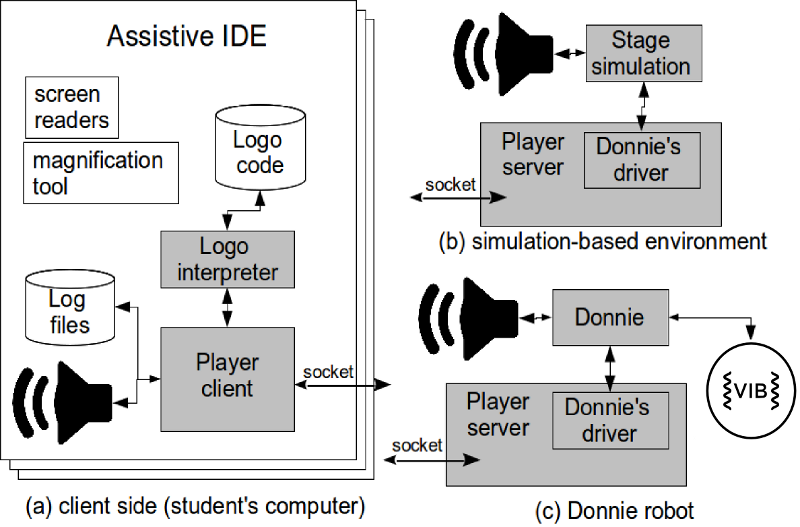
\includegraphics[width=0.95\linewidth]{figs/assistive-env.png}
  \caption{Donnie's system architecture.}
  \label{fig:donnie-sys}
\end{figure}


%%%%%%%%%%%%%%%%%%%%%%%%%%%%%%%%%%%%%%%%%%%%%%%%%%%%%%%

\subsection{Hardware Architecture}
\label{sec:hardware}

The hardware architecture consists of an open mechanical model \footnote{\url{https://github.com/lsa-pucrs/donnie-assistive-robot-3d}}, which can be built with a 3D printer, and an open electronic system \footnote{\url{https://github.com/lsa-pucrs/donnie-assistive-robot-hw}} based on Raspberry Pi and Arduino. Both boards were chosen due to their availability in the market, low cost, and the size of the developer community, which eases the addition of new capabilities in the future. Moreover, both boards are used in several educational projects, thus, the schools might already have some of these boards.

\subsubsection{The Mechanical Model}
\label{sec:mech}

Figure~\ref{fig:donnie-mech} illustrates Donnie's mechanical model and an example of 3D printed robot. Its main mechanical features include:

\begin{itemize}
\item It is a differential robot with two parallel wheels;
\item It has one bumper in the front and another in the rear;
\item It has a head that can turn to left and right-hand sides to scan the surroundings;
\item It has seven sonar sensors for obstacle avoidance;
\item It has a modular design, divided into stacks, such that an additional stack can be added on demand.
\end{itemize}



\begin{figure}[h!]
    \centering
    \begin{subfigure}[b]{0.8\linewidth}
        \centering
        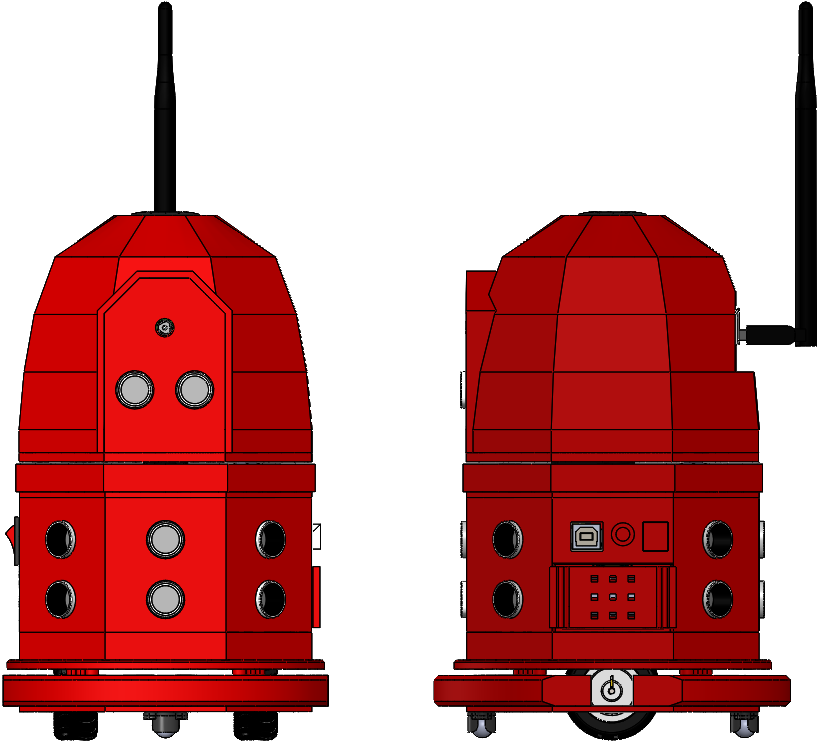
\includegraphics[width=\linewidth]{figs/donnie-3d_model.png}
        \caption{3D model.}
    \end{subfigure}
    ~
    \begin{subfigure}[b]{0.8\linewidth}
        \centering
        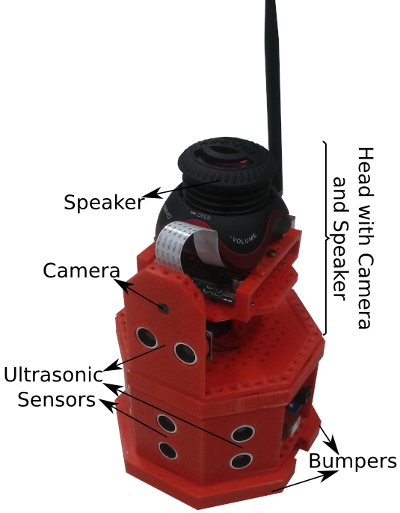
\includegraphics[width=\linewidth]{figs/donnie-printed.png}
        \caption{3D printed robot.}
    \end{subfigure}
    \caption{Donnie's mechanical model.}
    \label{fig:donnie-mech}
\end{figure}


%\begin{figure}[h!]
%  \centering
%    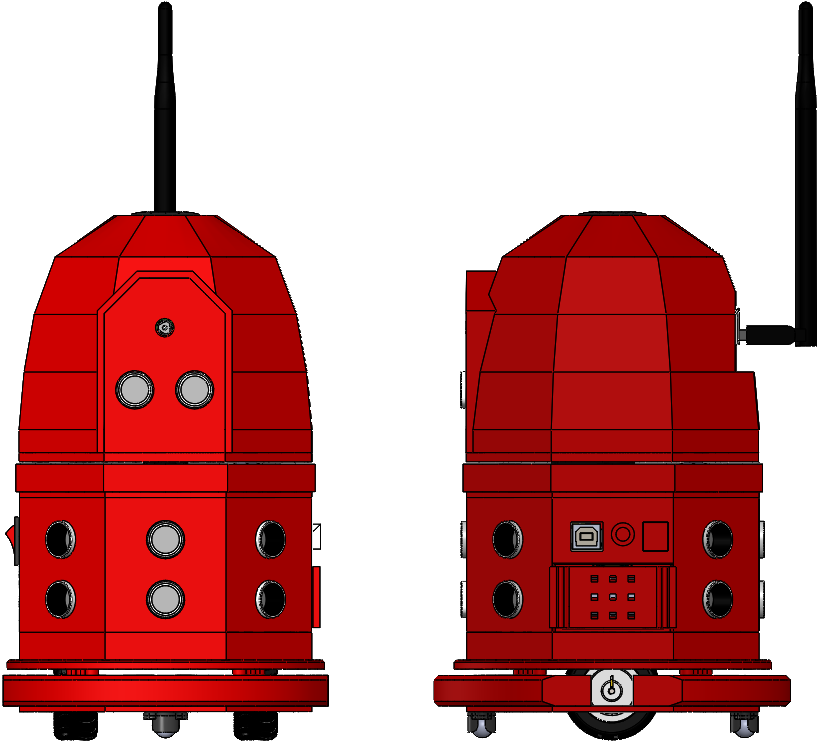
\includegraphics[width=0.5\textwidth]{figs/donnie-3d_model.png}
%  \caption{Donnie`s 3D Model.}
%  \label{fig:donnie-3d_model}
%\end{figure}

Currently Donnie has three stacks. The lower stack (the feet) is for the wheels, the motors, the motor encoders, and the bumpers. The second stack (the body) has the battery, six ultrasonic sensors, and the Arduino board. The third one (the head) has one ultrasonic sensor, the camera, the speaker, and the Raspberry Pi board. Additional stacks can be mounted in between the existing stacks to add new functionality.

%%%%%%%%%%%%

\subsubsection{The Electronic System}
\label{sec:elet}

Figure~\ref{fig:donnie-elet} illustrates Donnie's electronic systems which is divided in two main parts: Arduino and Raspberry Pi (RPi). While the RPi board does the interface to the robot`s peripheral which are similar to a computer peripheral (i.e. camera, speaker, wifi), the Arduino board does the interface to the IO resources exclusive for robots (range sensors, motors, encoders, etc). 

\begin{figure}[h!]
  \centering
    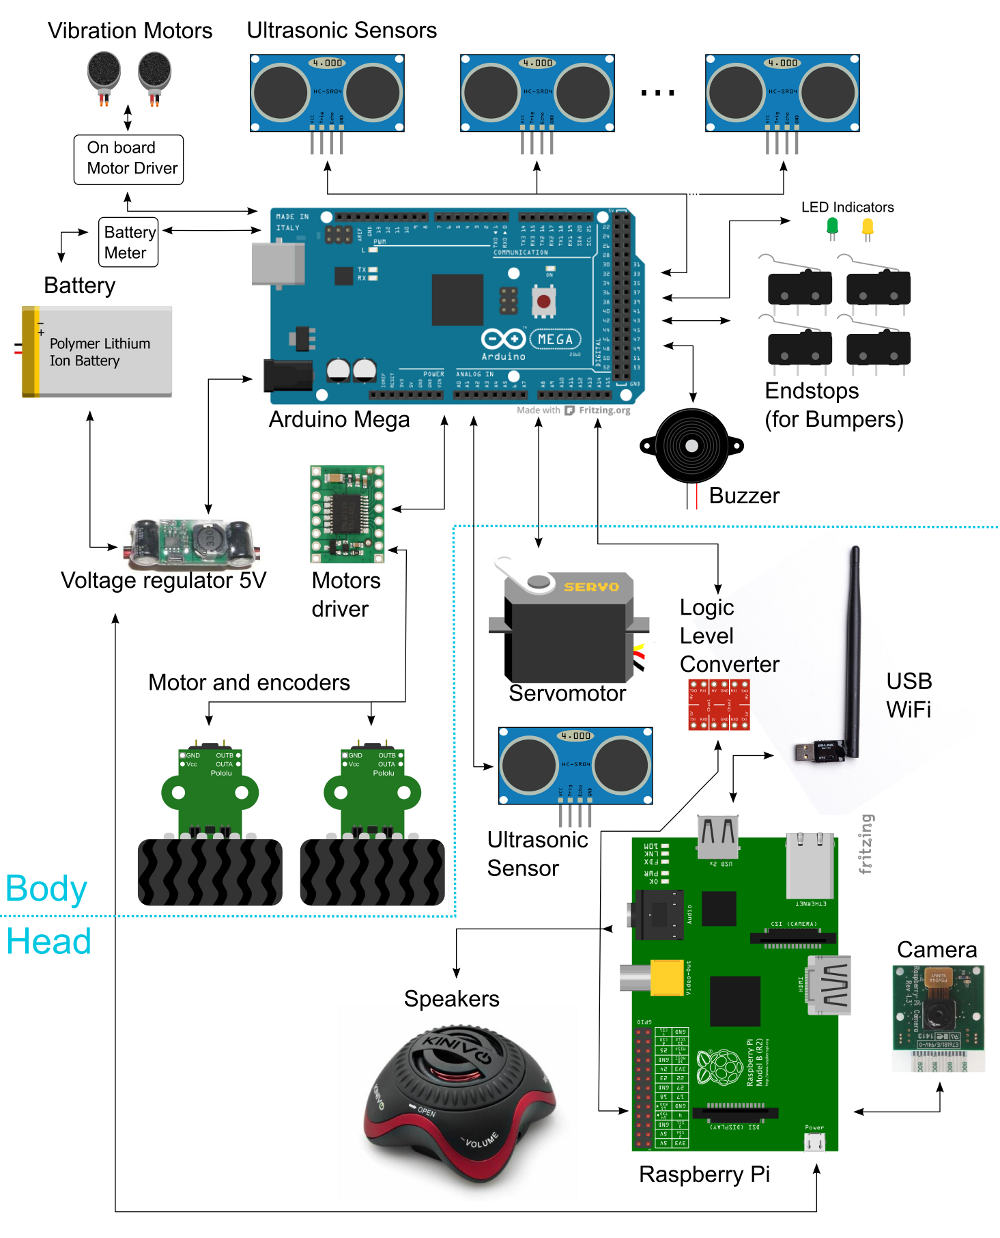
\includegraphics[width=0.95\linewidth]{figs/donnie-elet.png}
  \caption{Donnie's Electronic System: (a) Arduino and (b) Raspberry Pi.}
  \label{fig:donnie-elet}
\end{figure}

The design decision to use two boards (Arduino and RPi) instead of only one of them is discussed as follows. For instance, it would be possible to implement all peripherals using only the RPi board. However, this would lead to a reduced number of interfaces for future expansions and add-ons. By using an Arduino Mega, there are enough interfaces for several new features such as, for example, a gripper, line following sensors, among other possible extensions. Alternatively, there are few expansion boards for RPi for robotics \footnote{\url{https://www.adafruit.com/products/1940}} \footnote{\url{https://www.piborg.org/picoborgrev}} that could also be used instead of the Arduino Mega. The advantage of Arduino is its availability, large user community, and it can be removed from the robot and used alone to teach programming \cite{ardu-book1,ardu-book2}. This way, Arduino is a more versatile option than the RPi expansion boards. On the other hand, there are also several robot proposal using only Arduino boards. The main drawback of these approaches is that they provide limited computing capability, limiting the learning experience. The robot would become obsolete as soon as the student acquire the basic programming skill enabled by an Arduino board. This way, by combining both Arduino and RPi boards the robot become modular, expandable, and also with good computing capabilities to enable advanced programming and robotics learning. Both boards are also well documented, with several books about robotics such as \cite{rpi-book1,rpi-book2,rpi-book3} and \cite{ardu-book1, ardu-book2}.

As illustrated in Figure~\ref{fig:donnie-elet}, the Arduino board communicates with the Raspberry Pi board using the serial interface via a level shifter. The firmware running on the Arduino is explained in Section~\ref{sec:firm}. As illustrated in Figure~\ref{fig:donnie-elet}, the Arduino board is located at the robot's body and it controls:

\begin{enumerate}
\item The DC driver and two motors to move the robot;
\item The motor encoders that evaluate the distance travelled by each motor;
\item The buzzer and the vibrating motor used for assistive interface in case of robot collision, obstacle detection, low battery alert;
\item The LEDs provide similar feedback as mentioned before for students with normal vision;
\item The two tactile bump sensors, each one using two switches, used to detect collisions; 
\item The battery sensor used to indicate low battery;
\item The servo motor to implement the head movement for scanning the surroundings with head`s sonar and the camera (RaspiCam v1 with OmniVision OV5647 Color CMOS sensor);
\item Seven sonar sensors (including the one in the head) for navigation and obstacle avoidance;
\item The level shifter to adapt the serial voltage between the Arduino and the RPi boards.
\end{enumerate}

The Raspberry Pi board runs a Linux operating system with Raspbian distribution. This board runs the Donnie's device driver (Section~\ref{sec:driver}) and it also controls the camera (and its image processing), the sound at the speaker, and the wifi connectivity. 


%\todo{Marques e Augusto: falar das placas desenvolvidas. Favor preencher estas informações}

Two additional boards were developed to connect the robot's electrical components. The first board is a 3.6 by 4.2 cm board, with two layers, used to connect the RPi board with the electronics in the head (ultrasonic sensor and servo motor) with the Arduino board. The second board is attached to the Arduino board. It has 6.3 by 10.6 cm and two layers. It contains six ultrasonic connectors, two vibration motor drivers, one battery voltage meter, four digital bumper inputs, two leds, one buzzer output, two encoder inputs, and a motor driver to control two DC motors. This board has a connector to communicate with the first board. Both boards are illustrated in Figure~\ref{fig:donnie-boards}.


\begin{figure}[h!]
    \centering
    \begin{subfigure}[b]{0.60\linewidth}
        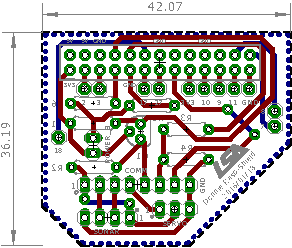
\includegraphics[width=\linewidth]{figs/rasp_shield_v1_eagle_brd.pdf}
        \caption{RPi board Layout.}
    \end{subfigure} %
    \begin{subfigure}[b]{0.85\linewidth}
        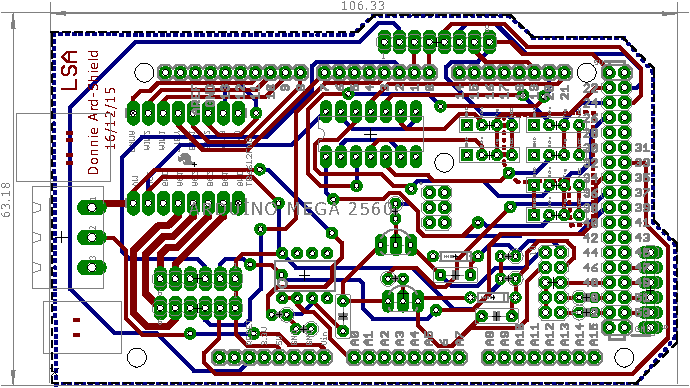
\includegraphics[width=\linewidth]{figs/arduino_shield_v1_eagle_brd.pdf}
        \caption{Arduino board Layout.}
    \end{subfigure}
%    \begin{subfigure}[b]{0.45\linewidth}
%        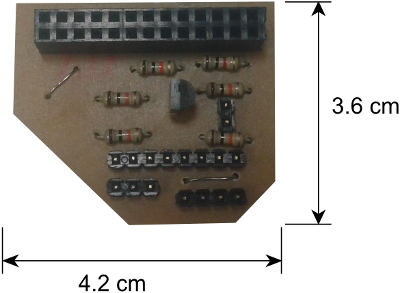
\includegraphics[width=\linewidth]{figs/rasp_board_v1.png}
%        \caption{Photo of the RPi board.}
%    \end{subfigure}
%    %\hspace{\fill} %
%    \hspace*{-0.6em} %
%    \begin{subfigure}[b]{0.45\linewidth}
%        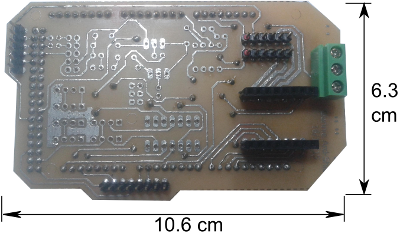
\includegraphics[width=\linewidth]{figs/arduino_board_v1.png}
%        \caption{Photo of the Arduino board.}
%    \end{subfigure}    
    \caption{Donnie's auxiliar boards.}
    \label{fig:donnie-boards}
\end{figure}



%%%%%%%%%%%%

\subsubsection{The Hardware Cost}
\label{sec:hw-cost}

The estimated cost to build a Donnie robot is US\$ 255 in electronics assuming none of the parts listed before are available. The amount of plastic required for 3D printing the robot is about 0.44 Kg. Assuming the plastic costs US\$48 per Kilo, the 3D printing cost is US\$ 21. 

The Table~\ref{tab:cost-table} shows the price of each component used to build Donnie, compared with the price of the equivalent parts of Lego's Mindstorms. The 'X' represents that the Lego does not have an equivalent official part and the '-' represents the item is not needed because it is included into the main part. For example, the Brick Mindstorm, that is build with an ARM9 micro processor, has an embedded speaker and Wi-Fi support, thus, it is not required to buy a separate piece. 
Few accessories were required to make Lego's Mindstorms more comparable with Donnie. Even though, Donnie still has advantages such as a better processor (able to run more complex codes and image processing), it has more sensors than Lego's robot, and it costs half the cost of an equivalent Lego's robot. 


\begin{table}[ht!]
\centering
\caption{The price table of Donnie's parts in comparison with Lego's Mindstorms equivalent parts.}
\label{tab:cost-table}
\begin{tabular}{|l|c|c|}
\hline
 & Donnie (U\$)    & Lego Mindstorms (U\$)  \\ \hline
motor driver             & 8.95    & -      \\ \hline
motor, encoder and wheel & 39.95   & 24.99  \\ \hline
micro controller         & 37.09   & 179.99 \\ \hline
servo                    & 19.95   & 19.99  \\ \hline
buzzer                   & 1.49    & X      \\ \hline
ultrasonic sensors       & 7*2.50  & 7*19.99\\ \hline
raspberry pi B           & 39.90   & X      \\ \hline
ubec                     & 5.98    & -      \\ \hline
camera                   & 29.95   & X      \\ \hline
usb wifi                 & 19.05   & -      \\ \hline
bumpers                  & 4*1.99  & 4*24.99\\ \hline
battery                  & 14.86   & 79.99  \\ \hline
speaker                  & 12.99   & -      \\ \hline
plastic                  & 21.00   & -      \\ \hline
\textbf{TOTAL (U\$)}     & \textbf{276.62} & \textbf{544.85}           \\ \hline
\end{tabular}
\end{table}


\subsection{Software Architecture}
\label{sec:software}

This section presents the open software architecture of the proposed system \footnote{\url{https://github.com/lsa-pucrs/donnie-assistive-robot-sw}}. We adopt a top-down presentation approach, initially presenting a discussion about choosing an appropriate programming language for people with visual disability. Next, we discuss the developed 
%assistive IDE, the 
graphical simulation environment, the driver interfacing the student`s computer and the robot, and the firmware embedded into the robot. 
The layered software architecture illustrated in Figure~\ref{fig:donnie-soft-layer} is built such that it invites the students, as they evolve in their programming skills, to gradually start coding also for the lower layers, improving their understanding of a complete computing software stack. 

\begin{figure}[h!]
  \centering
    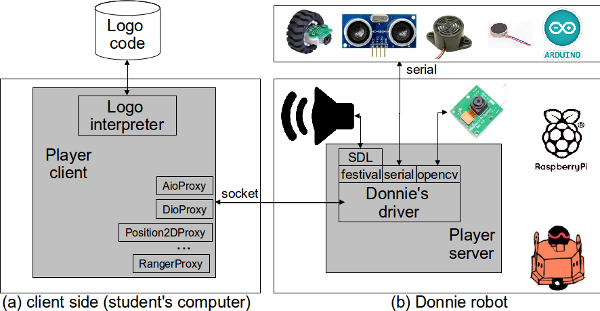
\includegraphics[width=0.95\linewidth]{figs/assistive-sw.png}
  \caption{Donnie's layered software stack.}
  \label{fig:donnie-soft-layer}
\end{figure}

As it is discussed later, novice students start coding with an ease to learn language for educational purposes (e.g. Logo). As this initial language starts to present limitations for the learning processes, it can be replaced for other languages with intuitive syntax (e.g. Ruby, Python), to finally move to more complex and complete languages such as C, C++, and Java. Currently, the Player robotic framework supports all languages mentioned before and it also has extensions to other more domain-specific languages such as Matlab \footnote{\url{http://playerstage.sourceforge.net/wiki/PlayerClientLibraries}} for numerical computing and Erlang \cite{Gruner:2009} for distributed systems. To the best of our knowledge, this is the first proposal of an educational language, similar to Logo, for Player. Moreover, thanks to the reuse of Player, this is the first assistive programming framework for robotics that supports so many languages.

In addition, the proposed system can also be used to teach multiple concepts of Computer Science, such as embedded programming, serial protocol, hardware/software interface, networked communication, topics of artificial intelligence (e.g. path finding, autonomous behavior), and computer vision (e.g. blob finder, tag recognition, pattern recognition), and advanced robotics (e.g. visual odometry, localization, mapping, multi-agent systems). Although at this stage of the project we are going to focus to teach programming to young students, the proposed system could also be used for high-school and graduate courses.

A crucial design decision was whether we would include a robotic software framework or not, and which framework to adopt. Current survey papers \cite{kramer2007,elkady2012} list dozens of robotic frameworks such as ROS, Orocos, Player, among others. The decision to support a framework was straight-forward since it enables to reuse useful codes (drivers and algorithms) to the proposed system. The second decision was which framework to adopt. Currently, ROS is probably the most used, documented, and with the biggest developer community \cite{quigley2009}. However, ROS is too complex for educational purposes, specially for students with little or none programming background. 

Player \cite{gerkey2003}, on the other hand, is much simpler in several aspects. First, it is based on a simpler client-server software design approach, compared to peer-to-peer, enabling simpler software design and hardware abstraction. The computational requirements to run Player is very low, which would fit nicely on an embedded processor. The source code is small (about 5 MBytes), the compilation process is straight-forward (few dependencies), there are several examples of robot drivers (there are dozen robots compatible with Player), and ready-to-use drivers for most common robotic resources (laser rangers, cameras, etc), it uses a simple textual configuration file to describe the robot drivers. Finally, Player/Stage are very active in the research community with currently more than 1500 citations just to the first paper \cite{gerkey2003}.

\subsubsection{Programming Languages}
\label{sec:prog-lang}

Choosing the initial programming language for young students with visual disabilities is an open problem. It has been reported that some languages are more difficult to students with visual disabilities. For example, Python uses whitespaces to delimit code blocks, which is hard to navigate with screen readers \cite{kane2014}. Languages such as C and Java use brackets to delimit code blocks, however, when the block is large with several sub-blocks, students with visual disabilities have difficult to find missing brackets.

The proposed system uses a Logo-based programming language because it was developed for educational context. Thus, the use of the Logo programming language is supported by a teaching methodology and an educational philosophy, which proposes the use of computers as a tool in the educational process~\cite{Valente1996}. To facilitate communication with the user, Logo commands are similar to natural language.

A new Logo-based language, called GoDonnie, is proposed to map the robot's capabilities. The complete specification of the language is presented in Table~\ref{tab:donnie-cmd}\footnote{GoDonnie language will be available in Portuguese and English.} and some examples of Portuguese commands are described below:


\begin{itemize}[topsep=0pt,itemsep=0ex,partopsep=0ex,parsep=0ex]
    \item Movement Commands:
    \begin{description}[topsep=0pt,itemsep=-1ex,partopsep=1ex,parsep=1ex]
        \item [PF:] It moves the robot forward for \textit{n} steps.
        \item [PT:] It moves the robot backwards for \textit{n} steps.
        \item [GD:] It spins the robot \textit{d} degrees to the right.
        \item [GE:] It spins the robot \textit{d} degrees to the left.
    \end{description}
    \item Selection Commands: 
    \begin{description}[topsep=0pt,itemsep=-1ex,partopsep=1ex,parsep=1ex]
        \item [SE:] It selects the code block to be executed based on the boolean value of a predicate.
    \end{description}
    \item Loop Commands: 
    \begin{description}[topsep=0pt,itemsep=-1ex,partopsep=1ex,parsep=1ex]
        \item [PARA:] It has three parts: variable initialization; loop condition;  increment the initialized variable. While the condition is true the robot executes the code block.
        \item [REPITA:] It repeats the code block \textit{t} times.
    \end{description}
    \item Position and Perception Commands:
    \begin{description}[topsep=0pt,itemsep=-1ex,partopsep=1ex,parsep=1ex]
        \item [CORES:] It returns the number of objects of a determined color \textit{c}.
        \item [ESPIAR:] It scans objects in $180^{o}$ in front of the robot. Then it returns the color, the distance, and the angle to the detected objects.
        \item [DISTÂNCIA:] The robot has six range sensors to measure the distance from obstacles. This command returns  the distance of the sensor \textit{r} to an object in steps.
        \item [ESTADO:] It returns series of current information about the robot such as its current pose, and the last instruction.
        \item [POS:] It returns the Cartesian \textit{X}, \textit{Y}, or angle \textit{A}.
    \end{description}
    \item Audio Commands:
    \begin{description}[topsep=0pt,itemsep=-1ex,partopsep=1ex,parsep=1ex]
        \item [SOM:] It turns on or off the robot sounds.
        \item [BIP:] It makes a noise in a chosen tone \textit{t} and period of time \textit{d}.
        \item [FALAR:] It speaks a phrase or word \textit{w} using a TTS.
    \end{description}
    \item Procedure Command:
    \begin{description}[topsep=0pt,itemsep=-1ex,partopsep=1ex,parsep=1ex]
        \item [APRENDER:] It implements procedures with an arbitrary number of arguments. This procedure can be called from any point of the program.
    \end{description}
\end{itemize}

More commands and usage information can be found in appendix A.

%\subsection{Assistive IDE}
%\label{sec:assit-ide}

%The developed IDE with textual interface is compatible with screen readers and magnification software. The IDE also has menus and shortcut keys to ease navigation; it narrates the debug log files, 

%\todo{INCLUIR FEATURES. Acredito que esta secao deva ser removida pois desenvolvemos muito pouco neste assunto.}

%\begin{figure}[h!]
%  \centering
%    
\includegraphics[width=0.5\textwidth]{figs/blank.jpg}
%  \caption{Assistive IDE screenshot.}
%  \label{fig:donnie-ide}
%\end{figure}

%%%%

\subsubsection{Graphical Simulation Environment}
\label{sec:simul}

The Player robotic framework is compatible with a lightweight 2D graphical simulation environment for multi robots called Stage \cite{Vaughan:2008}. This simulation environment is an option when the physical robots are not available. The main advantage is that the student`s software code does not change when the user migrates from virtual to physical robots or vice versa.
Stage simulates a population of multiple mobile robots, sensors and objects in a scene. It is designed to provide a computationally cheap and simple models of various devices, instead of trying to simulate devices with great fidelity. For this reason the Stage can simulate hundreds of robots in the same environment \cite{Vaughan:2008}, a feature that could be used for educational purposes, like in competition among the students where each student controls a robot and all robots share the same environment. 

The student can choose to use the simulated or the real robot, if this is available. We built Donnie's simulation models to be as close as possible to the real robot (Figure~\ref{fig:stage}(a)) such that the student can start debugging the software with simulation and use the real robot latter, when the code is more stable. Since Stage is graphical, we added sound to the robot's actions such that the students with visual disabilities can follow the steps of the robot. This feature is described in the next section.

The Figure~\ref{fig:stage}(b) shows a Stage screenshot, with one of the scenarios used for teaching that represents a room with one person, few tables, and sofas. A Stage scenario is described in a text file, with a simple syntax that enable students to create their own scenarios. The only non-textual part of a scenario definition is the description of the walls. This part requires drawing the walls with a software like Paintbrush, as illustrated in Figure~\ref{fig:stage}(c). %The students with visual disabilities receive also a floorplan of the scenario with Braille and tactile transcriptions of the environment (Figure~\ref{fig:stage}(c)). Then, the student is, for example, asked to find an object in the room. 


\begin{figure}[h!]
    \centering
    \begin{subfigure}[b]{0.7\linewidth}
        \centering
        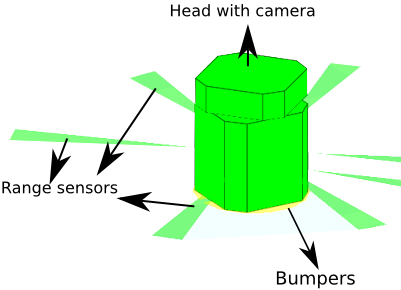
\includegraphics[width=\linewidth]{figs/donnie-simul.png}
        \caption{Donnie's virtual model.}
        \label{fig:donnie-simul}
    \end{subfigure}

    \begin{subfigure}[b]{0.7\linewidth}
        \centering
        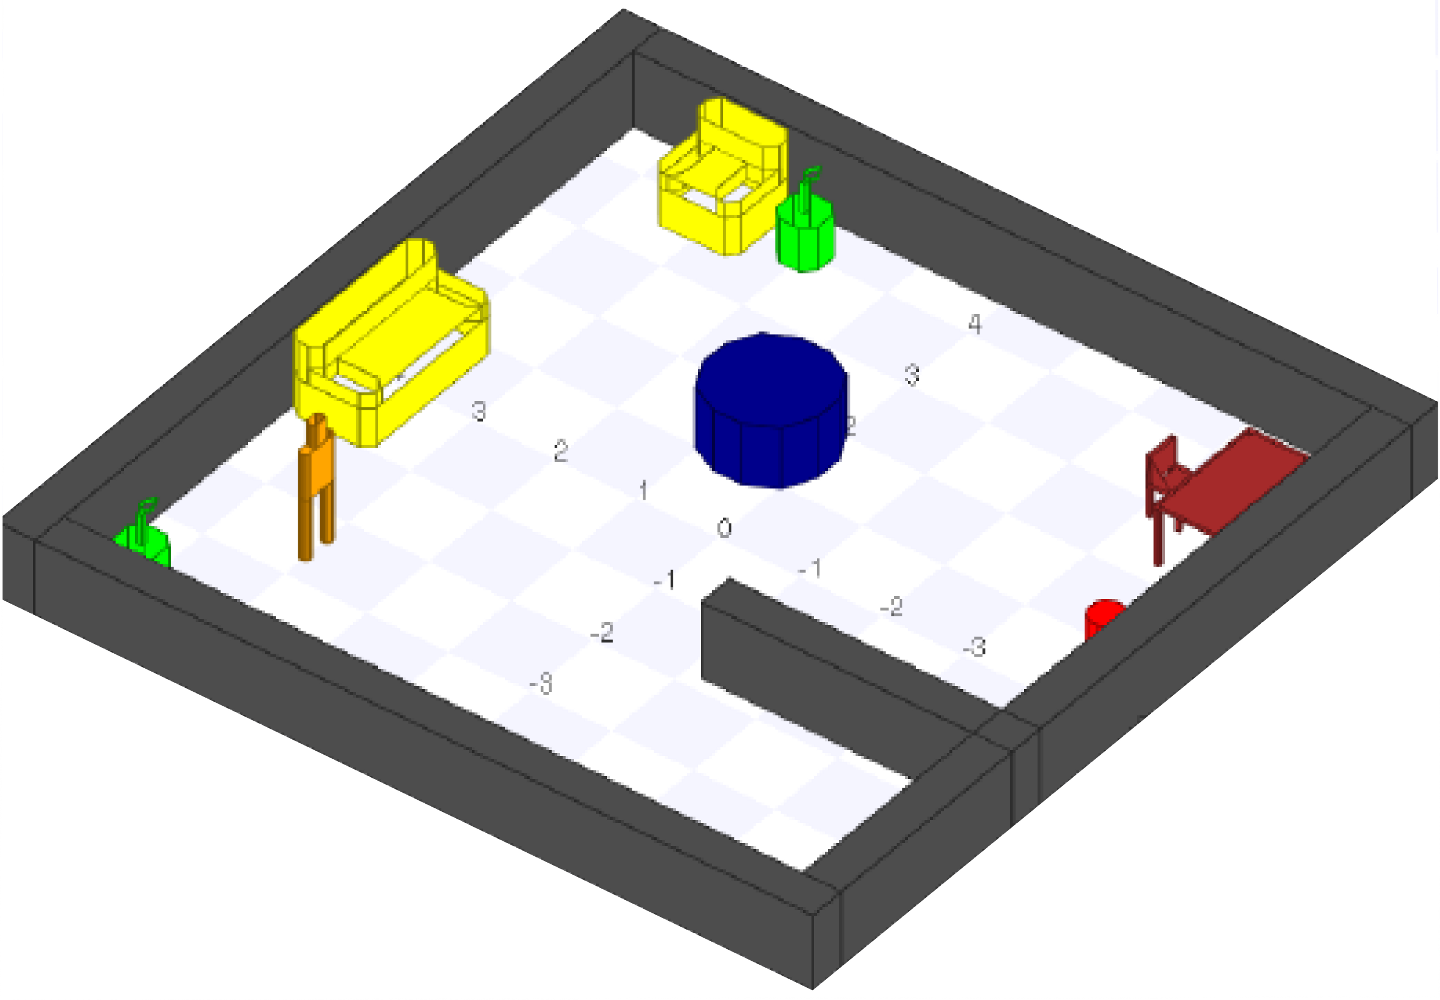
\includegraphics[width=\linewidth]{figs/stage-env.png}
        \caption{Screenshot of a Stage scenario.}
        \label{fig:stage-screen}
    \end{subfigure}

    %\begin{subfigure}[b]{0.47\linewidth}
    %    \centering
    %    
\includegraphics[width=\linewidth]{figs/blank.jpg}
    %    \caption{Braille and tactile description.}
    %    \label{fig:five over x}
    %\end{subfigure}
    
        \begin{subfigure}[b]{0.7\linewidth}
        \centering
        
\includegraphics[width=0.8\linewidth]{figs/mapa-stage.png}
        \caption{The png file for drawing the walls.}
        \label{fig:stage-wall}
    \end{subfigure}

    \caption{Stage-based virtual environment}
    \label{fig:stage}
\end{figure}


%%%%

\subsubsection{Donnie's Device Driver}
\label{sec:driver}

The Donnie's driver running on the RPi board is a Player driver~\cite{vaughan2007}, which connects the clients (student's computers) with the robot (either virtual or physical robot). It abstracts from the client software how the hardware resources are accessed. For example, the student can call a proxy interface called RangeProxy to read data from the sonar ring. It abstracts which low-level protocol is actually used, the brand of sensor, etc. Player has a set of predefined proxy interfaces~\cite{vaughan2007} for the most common robot resources like range sensors, cameras, grippers, motors, position, map, among dozens of other interfaces available. 

A Player driver is a piece of software used to remotely access the robot using these proxy interfaces. Donnie's Player driver uses the following set of existing interfaces:

\begin{itemize}
\item Position2d: used both to move and to get the robot's position;
\item Ranger: used to access the ring of seven ultrasonic sensors;
\item Blobfinder: returns a list of blobs capture in the image frames;
\item Dio (Digital IO): interface to read and write binary devices such as LEDs, buzzer, vibration motors;
\item Power: interface used to read battery status;
\item Bumper: detects collision from the bumper sensors;
\item Aio (Analog IO): interface to read and write analog devices such as light intensity sensor.
\end{itemize}

The following set of interfaces are under development:

\begin{itemize}
\item Speech: performs text synthesis with Festival text-to-speech \cite{black2001} and Google TTS;
\item Audio: plays various audio formats with the Sound eXchange (SoX) library \footnote{\url{http://sox.sourceforge.net/libsox.html}};
\item PiCamPlayer: A new Player driver to grab image frames from the RaspiCam;
\item BlobFinder: An updated Player driver, based on OpenCV 3.0, to detect blobs from cameras.
\end{itemize}

%\todo{Amory: A lista esta completa só nao tem o proxy speech e nem o proxy audio. O proxy AIO serviria para ler um sensor diverso tipo LDR ou um sensor de intensidade campo magnetico (Efeito Hall) mas não estamos usando isso no momento então eu tirei. Também não temos um proxy para line follower entao seria usado o DIO para isso.}

As illustrated in Figure~\ref{fig:donnie-soft-layer}, the requests to the interfaces position2d, ranger, among others are actually implemented in the Arduino board. Thus, the Player driver only translates the serial protocol to/from remote wifi access using Player`s built-in methods. On the other hand, the request to camera, blobfinder, and sound interfaces are actually executed in the RPi board. 
%The camera-related interfaces uses OpenCV for image processing while the sound-related interface uses Simple DirectMedia Layer (SDL) \footnote{\url{www.libsdl.org}} to play .wav files and Festival text-to-speech \cite{black2001}.

\begin{lstlisting}[language=C,frame=lines,xleftmargin=5.0ex, caption={Player-based device driver.},label=lst:donnie-driver]  
arduino = Serial(cfg_serial_port)
// main loop
while(TRUE) {
    processIncomingData()
    ProcessMessages()
    usleep(10)
}
\end{lstlisting}


Listing~\ref{lst:donnie-driver} presents a simplified view of the driver structure. It`s main goal is to translate clients requests. It initially sets up the serial port (line 1). Then, in an infinite loop, it treats incoming data from the Arduino (line 4) as, for example, tick count from the wheels, and it treats the incoming client`s requests (line 5) as, updated range data. Each of these two main functions is just a big switch case for every message type coming from the Arduino or the client computer, respectively.

The device driver is also responsible for generating sound clues that enables the student to follow the robot's movement. 
There are three types of sounds that Donnie can issue: movement sounds, stall sounds, and voice feedback. When Donnie moves, both the simulation model and the physical robot, it makes a sound that features it's movement. For example, one sound for moving forward, other for moving backward, and turning left/right. The stall sound works in a similar way, giving a feedback for the user when the robot hits or detects a wall with its bumpers and range sensors. Donnie can also give a voice feedback to the user when certain commands are executed, like the status commands. All types of sounds and the spoken language can be selected in a readable textual configuration file. Festival TTS currently supports English or Spanish while Google TTS supports several languages, including Brazilian Portuguese. However, Google TTS can only be used when the robot has Internet connection.

%%%%

\subsubsection{Donnie's Arduino Firmware}
\label{sec:firm}

Listing~\ref{lst:donnie-firm} presents a simplified view of the firmware structure running on the Arduino board. The main initial loop (line 1 to 5) waits for an initial configuration packet sent from the Player driver to the Arduino via the serial port. The robot does not start until this configuration packet is received, however, the power status is checked to alert the battery status. The firmware has series of configurable parameters detailed below: 

\begin{itemize}
\item PID parameters;
\item individual sensor update frequencies;
\item battery status parameters;
\item configurable pin ports.
\end{itemize}

%\todo{amory: esses sao os parametros que estamos usando by marques}

\begin{lstlisting}[language=C,frame=lines,xleftmargin=5.0ex, caption={Arduino-based firmaware.},label=lst:donnie-firm]  
do{
  sendRequestConfig() //request a robot config from driver
  cmd = readCommand() //receive robot config
  power_update() //check battery status
}while(cmd != CONFIGPACK) // wait until robot config received

// main loop
while(TRUE) {
  cmd = readCommand()  //Read incoming command from serial port
  processCommand(cmd)  //Execute requested command
  updateSensors()  //Read each sensor and update variables
  updateIndicators()  //Update leds, vibs and buzzer indicators
  sendData() //Send data to serial port
  updateTicks()  //Increment the tickCnt each 1ms (1000us)
}
\end{lstlisting}


The main loop in Listing~\ref{lst:donnie-firm} (lines 8 to 15) performs the robot control. It initially reads incoming packets from the serial port (line 9), it executes the commands (line 10) (e.g. move commands), it updates the sensor readings (line 11) into the internal memory, it updates the indicators (LEDs, buzzer, vibration motors) based on the command and sensor readings (line 12), and it sends the new data (line 13) via serial port to the Player Driver. 

%processCommand(cmd) {  
%	SWITCH(cmd){
%		CASE PINGPACK:
%			...
%		CASE DIOPACK:
%			...
%		CASE MOTORPACK:
%			...
%	}
%}
%
%void updateSensors(){
%	IF(tickCnt % UPDATE_DIO_FRQ == 0){
%		...
%	}
%	IF(tickCnt % UPDATE_RANGER_FRQ == 0){
%		ranger_update();
%	}
%	IF(tickCnt % 200 == 0){
%		power_update(tickCnt);
%	}
%	bumper_update();
%}
%
%
%sendData(){
%
%	IF(tickCnt % SEND_DIO_FRQ == 0){
%		sendSystemDioMsg(systemDio_data,5);
%	}
%	IF(tickCnt % SEND_RANGER_FRQ == 0){
%		sendRangerMsg(range,6);
%	}
%	IF(tickCnt % SEND_BUMPER_FRQ == 0){
%		sendBumperMsg(bumper,6);
%	}
%	IF(tickCnt % SEND_POWER_FRQ == 0){
%		sendPowerMsg(power);
%	}
%	IF(tickCnt % SEND_PING_FRQ == 0){
%		sendPing();
%	}
%}
%
%sendPowerMsg(data){
%    tx_data[0]=POWERPACK
%    tx_data[1]=lowBytes(data)
%    tx_data[2]=HighBytes(data)
%    tx_data_count = 3
%    writeData(tx_data,tx_data_count)
%}
%

%%%%

\subsubsection{Serial Communication Protocol}
\label{sec:serial}


The interface between RPi and Arduino is via a serial port. This section describes its protocol, illustrated in Figure~\ref{fig:serial-format}. The serial communication is another software layer which could be explored for teaching the concepts of data transfer, latency, bandwidth, data serialization, the memory sizes of scalar types, binary data representation, and finite state machine for building the protocol.

The protocol format presented in Figure~\ref{fig:serial-format} has two constants bytes of header, one byte of packet length, one byte for message types, variable number of bytes for the payload, and a final byte with checksum. Each functionality in the Arduino board has a corresponding message type. The most relevant message types are presented in Table~\ref{tab:serial-protocol}.

\begin{figure}[h!]
  \centering
    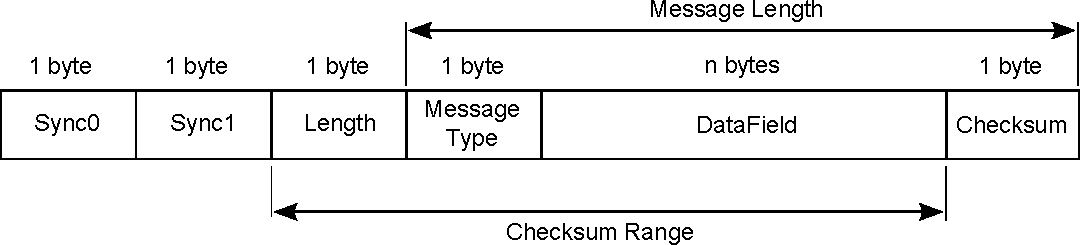
\includegraphics[width=0.45\textwidth]{figs/protocol.pdf}
  \caption{Serial packet format.}
  \label{fig:serial-format}
\end{figure}


\begin{table}[h]
  \caption{A sample of Donnie's serial communication protocol.}
  \label{tab:serial-protocol}
\begin{center}
  \begin{tabular}{ p{1.6cm} | p{3cm} | p{2.6cm} }
    \bf{message name} & \bf{description} & \bf{fields}\\
    \hline
    MOTORSTATE & defines direction and velocity for both motors & direction (left/right/on/off); right motor speed; left motor speed   \\
    \hline
    HEAD & defines the angular position of robot's head & mode (SCAN/SETPOS/GOTO); servo angle\\
    \hline
    RANGER & defines the 6 ultrasonic data & number of sensors; sensors data received \\
    \hline
    BUMPER & defines the 4 bumper data & number of sensors; sensors data received \\
    \hline
    POWER & defines the current battery voltage & float number indicating the measured voltage \\
    \hline
    ENCODER & defines wheel ticks from the wheel encoders & right wheel ticks; left wheel ticks \\
    \hline
    CONFIG & configures the micro-controller parameters using the parameters from a config file & any parameter defined in the config file (.cfg) \\
    \hline
    REQ\_CONFIG & requests from micro-controller for the parameters in the configuration file & none \\
    \hline
    REQ\_PING & requests from micro-controller to check the serial connection status & none \\
    \hline
    PING & used to check the serial connection status & none \\
    \hline
  \end{tabular}
\end{center}
\end{table}

When the student adds a new functionality to the robot, he/she has to define a new message type and adapt both the firmware and the driver to handle this new message.
The firmware and driver codes have comments to give clues to the students to find where to change.

\section{Usage Scenarios}
\label{sec:usage}


%	Explicar como as coisas funcionam… Integração…
%	Falar da detecção de cores…. (associar objetos a cor)
%	Falar do uso da aplicação com o “cercadinho” (pensar em um cenário de uso)
	
	
This section describes the assistive capabilities for users with visual disabilities. 

Starting with the software, this module allows a navigation free or based in scenarios. In free navigation, the user interacts only with the terminal and commands a virtual robot. All commands are perceived by the student via the computer's sound interface. The scenario-based navigation uses the robot and allows the user to send commands from the terminal to the robot, which will move into a space.
%Na navegação livre, o usuário interage somente com o terminal e comanda um robo virtual. Todos os comandos são transmitidos pela interface sonora. A navegação baseada em cenário utiliza o robô e permite que o usuário envie comandos pelo terminal ao robo, que se deslocará em um espaço. 

The hardware part of the system enables the robot to generate tactile and auditory feedback for students with visual disabilities. The speaker connected to the RPi board enables the robot to speak using Festival Google TTS text-to-speech software and to generate pre-configured sounds to indicate, for instance, collision, obstacle position/distance, robot steps, turns, object recognition, goal achievement, among other events. The buzzer and vibrating motors are used for more important alerts such as robot collision and low battery, which require immediate attention from the student.	

Stage enables the creation, for example, of a virtual arena where all student`s robots can be together by connecting to the same sever. This can be used to create competition where the robots must find an object in the arena, the robots have to collect objects (e.g. gold gems) from the environment, or the robots can interact with each other for cooperation and building teams.

%\pessoa vidente é aquele que enxerga. Utilizamos os termos person who is not blind ou person who is not visually impaired. Substitui as expressões "who is a seer" para "who is not blind".... Marcia

Some examples of usage scenarios are presented below:

\begin{itemize}
    \item Elias, who is not blind, is the father of Luiza, who is blind. Luiza begin their studies at a new school. So Elias uses the robot to teach the school space for Luiza. For this, he explains the basic commands of the robot and explains the school space. So asks to Luiza what the robot should do to get from one place to another in the school.
    % Elias, que é vidente, é pai de Luiza, que é cega. Luiza começará seus estudos em uma nova escola. Então, Elias utiliza o robô para ensinar o espaço da escola para Luiza. Para isso, ele explica os comandos básicos do robô e explica o espaço da escola. Então, pede para que a Luiza diga o que o robô deve fazer para ir de um lugar a outro da escola.
    
    \item John, who is blind, is typing commands while Luis, who is not blind, observes the robot running  in the real scenario. John is having trouble to take the robot to its destination because he is attentive to the lines of code that he is typing, forgetting the global context. Luis, who observes and monitors the movement of the robot, said that the robot is having trouble to reach the destination. John and Luis discuss how to solve the problem and to make the robot reaching the goal. For this, John selects the editor option that provides information about the setting and context where the robot is while Luis tells you what he is watching.
    % João, que é cego, está digitando os comandos enquanto Luis, que é vidente, observa a execução do robô no cenário real. João está com dificuldades para levar o robô ao seu destino porque está atento às linhas de código que está digitando, esquecendo-se do contexto global. Luis, que observa e acompanha a movimentação do robô, informa que o robô está com dificuldades para chegar ao destino. João e Luis discutem sobre como solucionar o problema e fazer com que o robô alcance o objetivo. Para isso, João seleciona a opção do editor que fornece informações sobre o contexto do cenário e onde se encontra o robô enquanto o Luis informa o que está observando.
    
    \item Amanda, who is not blind and beginner in programming, decides to program the robot. Mary, who is blind and already have programming knowledge, will help her. For this, Maria proposes a path to be executed by the robot and explains the basic commands for Amanda. After, Amanda begins to write the program while Mary accompanies with touch, the movement of the robot in the scenario and provides feedback to Amanda. After the robot reaches the goal, Amanda and Mary review the commands and the robot trajectory and discuss if they could optimize the schedule.
    % Amanda, que é vidente e iniciante em programação, decide programar o robô. Maria, que é cega e já tem conhecimento de programação, irá ajudá-la. Para isso, Maria propõe um trajeto para ser executado pelo robô e explica os comandos básicos para a Amanda. Após, Amanda começa a escrever o programa enquanto Maria acompanha, com o tato, a movimentação do robô no cenário e fornece feedback para a Amanda. Após o robô alcançar o objetivo, Amanda e Maria revisam os comandos e a trajetória do robô e discutem se poderiam otimizar a programação.
    
    \item Afonso and Anna, who are blind, will program the robot together. They use touch to recognize the scenario, the initial position of the robot, and the target position. They discuss and decide what commands they should use. Later, Afonso enters each command while Ana verifies if the result is the expected, according to the previously agreed path. Ana verifies that the robot did not do a desired path and asks Afonso to read the commands previously typed while she simulates the robot's movement with touch. Together they check the wrong program segment and restart the trajectory from the starting position.
    % Afonso e Ana, que são cegos, vão programar juntos o robô. Para isso, utilizando o tato, reconhecem o cenário, a posição inicial do robô e a posição de destino. Discutem e decidem que comandos vão utilizar. Após, o Afonso vai digitando cada comando enquanto a Ana verifica se o resultado é o esperado, de acordo com a trajetória previamente combinada. Ana verifica que o robô não fez um caminho desejado e pede para que o Afonso leia os comandos já digitados enquanto ela simula com o tato o movimento do robô. Em conjunto, verificam o trecho de programa que está errado e refazem a trajetória começando da posição inicial.
    

    \item Professor Gabriel teaches programming classes for a class that has sighted and blind students. He proposes an activity of program optimization. For this, he has developed a program which the robot goes from a starting point to the destination making several turns and passing close to 5 objects. The challenge to the students is to move the robot from the starting point to the destination using the shortest way, and passing close to only two objects. All students have explored the scenario only with the touch. So the seers students were blindfolded. Afterwards, the students discussed and built models to use as support for programming. Professor Gabriel explained their program and asked that the students, in groups of three students, rewrite the program. After the timeout, all programs were discussed and the group has chosen the best resolution.
    %O professor Gabriel ministra aulas de programação para uma turma que possui alunos videntes e alunos cegos. Ele propôs uma atividade de otimização de programa. Para isso, elaborou um programa que fazia o robô partir de um ponto inicial e chegar a um destino fazendo várias voltas e passando próximo a 5 objetos. O desafio imposto aos alunos foi de que fizessem o robô sair do ponto inicial e alcançasse o ponto final utilizando o menor trajeto, e passando próximo a somente 2 objetos. Todos os alunos exploraram o cenário somente com o tato. Por isso, os alunos videntes ficaram com os olhos vendados. Após, os alunos discutiram e construiram maquetes para utilizar como apoio à programação. O professor Gabriel explicou seu programa e pediu para que os alunos, em grupos de 3 alunos, reescrevessem o programa. Passado o tempo limite, todos os programas foram discutidos e a turma elegeu a melhor resolução.
    
    \item Ricardo, who is not blind, and Denise, who is blind, need to build a scenario of a particular museum. For this, they explore the virtual environment, they discuss and tell to the others where the objects that will represent the museum's experiments on the scene should be placed.
    % Ricardo, que é vidente, e Denise, que é cega, precisam construir um cenário de um determinado museu. Para isso, exploram o ambiente virtual, discutem e vão informando aos demais aonde devem ser colocados os objetos que irão representar os experimentos do museu no cenário.

\end{itemize}

\section{Conclusion and Future Work}
\label{sec:conclusion}

This paper presented a robotic programing environment, built with open hardware and software, that has been designed for people with normal vision and also for visual impaired people. The paper details the hardware, the firmware, the driver design, and the virtual simulation environment. Currently there is a Logo interpreter with sound feedback (text synthesis and event sounds) but it still requires additional design effort to integrate it with a screen reader and a magnification tool. Finally, we believe that the overall programing environment is almost complete and we are planning to start testing and evaluating it.

In the near future, we plan to evaluate the sound feedback for Stage with visual impairment users. It is unclear how effective this virtual environment will help to learn programming and if it is able to hold the student`s attention and curiosity for a long period. For this reason, we also plan to compare the system with virtual robots or the system with physical robots to check each one is more effective for the learning processes.

We also plan to evaluate if the environment helps the students to improve their O\&M and programming skills. 
%Para isso, está prevista a realização de testes piloto para validar a metodologia de uso da linguagem de programação e do uso do robô e para revisar o protocolo de avaliação de qualidade de uso do ambiente. 
We are planning test trials to validate the usage metodology of GoDonnie languague, the Donnie robot, and the quality assesment of the overall framework. 

%\section{Conclusion}
\label{sec:conclusion}





% use section* for acknowledgement
\section*{Acknowledgment}

This work was partially supported by PUCRS via projects BPA-PEC-DES 08/2016, BPA-PEC-DES 11/2015, BPA-PEC-DES 11/2014 and FACIN's 1/2013, and by CNPq via PIBIC undergraduate student grants.

% Can use something like this to put references on a page
% by themselves when using endfloat and the captionsoff option.
%\ifCLASSOPTIONcaptionsoff
%  \newpage
%\fi



% trigger a \newpage just before the given reference
% number - used to balance the columns on the last page
% adjust value as needed - may need to be readjusted if
% the document is modified later
%\IEEEtriggeratref{8}
% The "triggered" command can be changed if desired:
%\IEEEtriggercmd{\enlargethispage{-5in}}

% references section

% can use a bibliography generated by BibTeX as a .bbl file
% BibTeX documentation can be easily obtained at:
% http://www.ctan.org/tex-archive/biblio/bibtex/contrib/doc/
% The IEEEtran BibTeX style support page is at:
% http://www.michaelshell.org/tex/ieeetran/bibtex/
\bibliographystyle{IEEEtran}
\bibliography{main.bib}
% argument is your BibTeX string definitions and bibliography database(s)
%\bibliography{IEEEabrv,../bib/paper}
%
% <OR> manually copy in the resultant .bbl file
% set second argument of \begin to the number of references
% (used to reserve space for the reference number labels box)

% biography section
% 
% If you have an EPS/PDF photo (graphicx package needed) extra braces are
% needed around the contents of the optional argument to biography to prevent
% the LaTeX parser from getting confused when it sees the complicated
% \includegraphics command within an optional argument. (You could create
% your own custom macro containing the \includegraphics command to make things
% simpler here.)
%\begin{biography}[{\includegraphics[width=1in,height=1.25in,clip,keepaspectratio]{mshell}}]{Michael Shell}
% or if you just want to reserve a space for a photo:

%\begin{IEEEbiography}[{\includegraphics[width=1in,height=1.25in,clip,keepaspectratio]{picture}}]{John Doe}
%\blindtext
%\end{IEEEbiography}

% You can push biographies down or up by placing
% a \vfill before or after them. The appropriate
% use of \vfill depends on what kind of text is
% on the last page and whether or not the columns
% are being equalized.

%\vfill

% Can be used to pull up biographies so that the bottom of the last one
% is flush with the other column.
%\enlargethispage{-5in}

\begin{landscape}
\appendices
\section{Lista de comandos do GoDonnie}

% Imprime uma página indicando o início dos apêndices
% ----------------------------------------------------------

\begin{small}
\begin{longtable}{ p{3cm} p{3cm} p{8cm} p{8cm}}
\\
\label{tab:donnie-cmd}\\
\toprule
    \textbf{Comando} 
    & \textbf{Argumentos}  
    & \textbf{Explicação}  
    &\textbf{Exemplo}
\\ \hline
    \textbf{PF n}
    & n é o número de passos
    & Anda n passos para frente
    & PF 5 
    \newline

O robô andará 5 passos para frente. Supondo que o robô está na posição 0, 0 e virado para o norte, o comando PF 5 colocará o robô na posição 5, 0, mantendo a direção para o norte. 
\\ \hline
    \textbf{PT n}
    & n é o número de passos  
    & Anda n passos para trás. É como se andasse de ré.  
    & PT 5 
    \newline
    
    O robô andará 5 passos para trás. Supondo que o robô está na posição 5, 0 e virado para o norte, o comando PT 5 colocará o robô na posição 0, 0, mantendo a direção para o norte.  
\\ \hline
    \textbf{GD x}
    & x é número de graus 
    & Gira x graus para direita. Não há deslocamento do robô. 
    & GD 90
    \newline

    O robô irá girar 90 graus para direita. Supondo que o robô está virado para o norte, o comando GD 90 irá girar o robô 90 graus para a direita, mantendo-o na  direção leste.  
\\ \hline
    \textbf{GE x} 
    & x é número de graus 
    & Gira x graus para esquerda. Não há deslocamento do robô. 
    & GE 90
\newline

    O robô irá girar 90 graus para esquerda. Supondo que o robô está virado para o leste, o comando GE 90 irá girar o robô 90 graus para a esquerda, mantendo-o na  direção norte. 
\\ \hline
    \textbf{ESPIAR}
    & nenhum 
    & Retorna a identificação do objeto, um ângulo aproximado e a distância aproximada de colisão entre o robô e o objeto identificado. 
    \newline 
    O rastreamento para identificação dos objetos ocorre a 90º graus a esquerda e a direita da frente do robô. 
    & Supondo que o robô está na posição 2,3, virado para o norte, e que há um obstáculo verde na posição 0,5 e outro obstáculo vermelho na posição 6,3.
    \newline

    ESPIAR
    Resposta: verde, 40º a esquerda, 2 passos, vermelho, 90º a direita, 4 passos 
\\ \hline
    \textbf{DISTÂNCIA d}
    & d é a direção (f - frontal; fd - frontal direita; d - direita;  td - traseiro direito; t - traseiro; te - traseiro esquerda; e - esquerda; fe - frontal esquerda) 
    & Retorna a quantidade de passos do sensor do robô até um obstáculo, de acordo com a direção escolhida.
    \newline

    Distância F retorna o número de passos do robô até um objeto que foi detectado pelo sensor da parte da frente do robô. 
    \newline

    Distância FD retorna o número de passos do robô até um objeto que foi detectado pelo sensor da parte da frente lateral direita do robô. 
    \newline

    Distância TD retorna o número de passos do robô até um objeto que foi detectado pelo sensor da parte da trás lateral direita do robô.
    \newline

    Distância T retorna o número de passos do robô até um objeto que foi detectado pelo sensor da parte da traseira do robô. E, assim, sucessivamente.
    \newline

    Não havendo obstáculos, retorna a quantidade de passos que o sensor consegue identificar.
    &  
    DISTÂNCIA F
    DISTÂNCIA FD
    DISTÂNCIA FE
    DISTÂNCIA T
    DISTÂNCIA TE
    DISTÂNCIA TD
    \newline
    
    Supondo que o robô está na posição 0,0, virado para o norte e há obstáculos nas seguintes posições, o resultado será:
    \newline

    Obstáculo em 0, 3: 
    DISTÂNCIA F

    Resposta: 3 passos
\\ \hline
    \textbf{ESTADO}
    & nenhum & Informa a posição x e Y do robô no eixo cartesiano e último comando digitado, antes de Estado. 
    & PF 3 ESTADO
    \newline

    Supondo que o robô estava em 0,0. O robô andará 3 passos para frente e informará 0 3 PF 3.
    \newline

    Não havendo obstáculos, converter a distância máxima (3 metros) em passos. 
\\ \hline
    \textbf{CRIAR x}
    & x é uma variável que será criada 
    & Cria uma variável igual a um valor ou a uma expressão. Lembrar que ao criar uma variável novamente, ela irá sobrescrever o valor anterior. 
    & Exemplo 1: CRIAR A
    Cria uma variável chamada A.
    \newline

    A = 2
    Tendo sido criada a variável, pode atribuir um valor diretamente. A variável chamada A armazena 2.
    \newline

    CRIAR B =5
    Cria uma variável chamada B, que armazena o valor 5
    \newline

    CRIAR C = A + B
    Cria uma variável chamada C, que recebe o valor da variável A somado ao valor da variável chamada B. O resultado da variável C é 7.
    \newline
    
    C = 1
    Altera o valor da variável C e armazena o valor 1, perdendo o valor anterior.
    \newline

    D = 5
    Retornará erro porque a variável D ainda não foi criada. 
\\ \hline

    \textbf{POS k} 
    & k é um eixo do plano cartesiano (X ou Y) ou ângulo (A). 
    & Retorna a posição atual do robô no eixo X ou no eixo Y ou o ângulo atual do robô. & Supondo que o robô está na posição 0,0 virado para o norte:
    \newline
    
    PF 2

    GE 90

    PF 5

    POS X (retornará -5)

    POS Y (retornará 2)

    POS A (retornará 270)

    GD 90

    POS A (retornará 0) 

    GD 90 

    POS A (retornará 90)
\\ \hline
    \textbf{PARA inicialização; expressão operador lógico expressão; incremento ou decremento 
    FAÇA comandos FIM PARA}
    & Inicialização: variável  = algum valor inteiro

    variável ou Expressão operador lógico variável ou expressão:
    variável ou expressão - operador lógico - variável ou expressão
    
    Incremento: variável + constante ou variável + variável
    
    Decremento: variável - constante ou variável - variável & Repete os comandos enquanto  a Expressão-operador lógico-expressão for verdadeira. & Supondo que o robô está na posição 0,0, virado para o norte e precise fazer um quadrado de tamanho de lado 3.
    \newline

    PARA 
    
    a=1; a<=4; a=a+1 
    
    FAÇA  
    
    PF 3 GD 90 
    
    FIM PARA
    \newline

    Supondo que o robô comece na posição 0,0. A variável a começará com o valor 1 e repetirá os comandos PF 3 e GD 90 enquanto a variável a for menor ou igual a 4. Ao final, o robô terá feito um trajeto similar a um quadrado e finalizará na posição 0,0 virado para o norte. 
\\ \hline
    \textbf{REPITA n VEZES comandos FIM REPITA}
    & n é o número de vezes que os comandos serão repetidos.
    & Repete os comandos n vezes. 
    & 
    REPITA 4 VEZES 
    
    GD 90 
    
    PF 2 
    
    FIM REPITA
    \newline
    
    Supondo que o robô comece na posição 0,0. Os comandos PF 3  GD 90 serão repetidos 4 vezes. Ao final, o robô terá feito um trajeto similar a um quadrado e finalizará na posição 0,0 virado para o norte.
\\ \hline
    \textbf{SE expressão operador lógico expressão 
    ENTÃO comandos SENÃO comandos FIM SE}& expressão = variável ou expressão. 
    & Testa se uma condição é verdadeira e, em caso afirmativo, executa os primeiros comandos. Caso contrário, executa os comandos da expressão Senão. 
    & Supondo que, se a variável a for menor do que 4 o robô tenha que andar para frente 5 passos e caso contrário tenha que girar 45 graus para esquerda:
    \newline
    
    SE a\textless 4 
    
    ENTÃO PF 5 
    
    SENÃO GE 45
    
    FIM SE  
\\ \hline
    \textbf{BIP n, d}
    & n é a nota musical e d é a duração em segundos (do, ré, mi, fá, sol, lá, si) 
    & Faz o robô emitir um som de acordo com a nota musical que durará d segundos. Este som é emitido pelo robô ou pelo ambiente virtual, dependendo de quem estará ativo. 
    & 
    BIP do, 3
    
    BIP ré, 1
    
    BIP mi, 6
    
    BIP fá, 7
    
    BIP sol, 3
    
    BIP lá, 4
    
    BIP si, 9   
\\ \hline
    \textbf{SOM a}
    & a é o estado do áudio, que pode estar ligado ou desligado. 
    & Comando que liga ou desliga o áudio do recurso que estiver ativo, que poderá ser o robô ou o ambiente virtual. 
    & SOM LIGAR

    SOM DESLIGAR 
\\ \hline
    \textbf{APRENDER nome: variável1, variável2, variável3, … INICIO comandos FIM APRENDER}
    & nome é o nome da função e variavel1, variavel2, variavel3  são os argumentos da mesma 
    & É utilizado para “ensinar” comandos ao robô. &  O robô precisa executar vários retângulos de tamanhos diferentes. Para isso, pode ser criado um procedimento chamado RETÂNGULO que teria duas variáveis, uma para receber o tamanho da altura e outro o tamanho da base.  
    \newline   
       
    APRENDER RETÂNGULO: base, altura
    
    FAÇA
    
    PF base GD 90 
    
    PF altura
    
    GD 90 
    
    PF base 
    
    GD 90 
    
    PF altura 
    
    GD 90 
    
    FIM APRENDER
    \newline
    
    retângulo 5,3
    
    retângulo 8,4
    
    retângulo 9,5  
\\ \hline
    \textbf{FALAR x}
    &  x é uma palavra ou frase
    & Fala a palavra ou frase contida em x.  Este som é emitido pelo robô ou pelo ambiente virtual, dependendo de quem estará ativo.
    & FALAR “oi”
\\ \hline
    \textbf{ESPERAR x}
    & x é o tempo em segundos 
    & Espera x segundos para executar o próximo comando. 
    & Se o robô deve andar para frente 2 passos, esperar 3 segundos e andar mais 4 passos:
    \newline
        
    PF 2 
    
    ESPERAR 3
    
    PF 4 
\\ \hline
    \textbf{SAIR}
    & nenhum
    & Fecha o ambiente de programação. Só pode ser usado no terminal. 
    & SAIR
\\ \hline
    \textbf{HISTÓRICO}
    & nenhum
    & Lê o que está na tela. É possível navegar usando P, para ir para a próxima linha, A, para ir para a linha Anterior, ou pode pular para uma linha determinada. Para sair do histórico usa-se a tecla ESC.
    & Supondo que tenham sido escritos os seguintes comandos:
    \newline
        
    PF 3
    
    GD 45
    
    PF 6
    
    GD 45
    
    PF 3
    \newline
    
    HISTÓRICO
    
    “O programa tem 5 linhas. Você está na linha 6. Digite o número da linha desejada ou P para ir para a próxima linha ou A para ir para a linha Anterior ou ESC para sair do histórico".
    \newline
    
    P
    “Não existe comandos”
    
    A
    
    será falado PF 3
    
    A
    
    será falado GD 45
    
    1
    
    será falado PF 3
    
    ESC
    
    sairá do histórico
\\ \hline
    \textbf{CORES c}
    & c é a cor desejada (azul; vermelho; verde)
    & Verifica quantos objetos de determinada cor o robô consegue identificar na sua frente.
    & Supondo que há 1 objeto vermelho e 2 azuis
    \newline
    
    CORES vermelho
    
    será falado 1
    
    CORES azul
    
    será falado 2
\\ \hline
    \textbf{Operadores lógicos}
    &  
    + soma
    
    - subtração
    
    * multiplicação
    
    / divisão
    
    \textless\textgreater diferente
    
    == igual comparação
    
    = atribuição
    
    \textless menor
    
    \textgreater maior
    
    \textless= menor ou igual
    
    \textgreater= maior ou igual

    &  Operadores para comparar valores ou expressões.
    & 
\\ 
\bottomrule
\end{longtable}
\end{small}

\end{landscape}


% that's all folks
\end{document}
